% EZRA UDP Debugger — manual lengkap & panduan pengecekan di pabrik
% Build: latexmk -xelatex ezra-udp-debugger-manual.tex   (butuh font Carlito + DejaVu)
\documentclass[11pt,a4paper]{article}

\usepackage{fontspec}
\usepackage[a4paper,left=20mm,right=20mm,top=24mm,bottom=22mm,headheight=14pt]{geometry}
\usepackage{xcolor}
\usepackage{graphicx}
\usepackage{tikz}
\usetikzlibrary{arrows.meta,positioning,shapes.geometric,calc,fit,backgrounds}
\usepackage{booktabs,tabularx,xltabular,array,multirow}
\usepackage{enumitem}
\usepackage{titlesec}
\usepackage{fancyhdr}
\usepackage[most]{tcolorbox}
\usepackage{listings}
\usepackage[hidelinks]{hyperref}

% ------------------------------------------------------------------ fonts
\setmainfont{Carlito}            % metric-compatible Calibri = typeface logo EZRA
\setsansfont{Carlito}
\setmonofont{DejaVu Sans Mono}[Scale=0.82]
\newfontfamily\symfont{DejaVu Sans}

% ----------------------------------------------------------------- colors
\definecolor{ink}{HTML}{1C221E}
\definecolor{muted}{HTML}{5C655F}
\definecolor{faint}{HTML}{8A928C}
\definecolor{ezline}{HTML}{C4C9C2}
\definecolor{well}{HTML}{EBEDE8}
\definecolor{panel}{HTML}{F5F6F2}
\definecolor{signal}{HTML}{F2A900}
\definecolor{estop}{HTML}{C8201A}
\definecolor{lamp}{HTML}{1F8A55}
\definecolor{tx}{HTML}{1F6FB2}
\definecolor{rx}{HTML}{B2622A}
\definecolor{bsync}{HTML}{2B322E}
\definecolor{blen}{HTML}{1F6FB2}
\definecolor{bid}{HTML}{6A4FB0}
\definecolor{bfmt}{HTML}{138A86}
\definecolor{bseq}{HTML}{B2622A}
\definecolor{bver}{HTML}{6F7B2C}
\definecolor{bres}{HTML}{9BA39C}

\color{ink}
\hypersetup{colorlinks=true,linkcolor=tx,urlcolor=tx,citecolor=tx}

% ------------------------------------------------------------- layout etc
\setlength{\parindent}{0pt}
\setlength{\parskip}{5pt plus 1pt}
\linespread{1.08}
\setlist{itemsep=2pt,topsep=3pt,parsep=0pt,leftmargin=18pt}
\renewcommand{\contentsname}{Daftar isi}
\renewcommand{\figurename}{Gambar}
\renewcommand{\tablename}{Tabel}
\renewcommand{\arraystretch}{1.22}

\titleformat{\section}{\fontsize{19}{23}\selectfont\bfseries}{\color{signal!80!black}\thesection}{0.55em}{}[\vspace{1pt}{\color{ezline}\titlerule[0.8pt]}]
\titleformat{\subsection}{\fontsize{14}{17}\selectfont\bfseries}{\color{muted}\thesubsection}{0.5em}{}
\titleformat{\subsubsection}{\large\bfseries}{}{0em}{}
\titlespacing*{\section}{0pt}{14pt}{8pt}
\titlespacing*{\subsection}{0pt}{12pt}{5pt}
\titlespacing*{\subsubsection}{0pt}{9pt}{3pt}

\pagestyle{fancy}
\fancyhf{}
\fancyhead[L]{\small\color{muted}EZRA UDP Debugger --- manual lengkap}
\fancyhead[R]{\small\color{muted}v0.2.0 · Inspection Protocol V1.0.3}
\fancyfoot[C]{\small\color{muted}\thepage}
\renewcommand{\headrulewidth}{0.4pt}
\renewcommand{\headrule}{\hbox to\headwidth{\color{ezline}\leaders\hrule height \headrulewidth\hfill}}

% ---------------------------------------------------------------- helpers
\newcommand{\code}[1]{\texttt{#1}}
\newcommand{\cb}{{\symfont\large ☐}}
\newcommand{\ok}{{\symfont\color{lamp}✓}}
\newcommand{\no}{{\symfont\color{estop}✗}}
\newcommand{\ra}{\ensuremath{\rightarrow}}
\newcommand{\gear}{{\symfont ⚙}}
\newcommand{\ui}[1]{\textbf{#1}}
\newcommand{\tahap}[1]{\subsection*{#1}\addcontentsline{toc}{subsection}{#1}}
\newcolumntype{L}[1]{>{\raggedright\arraybackslash}p{#1}}
\newcolumntype{Y}{>{\raggedright\arraybackslash}X}

\tcbset{boxrule=0.6pt,arc=2pt,left=7pt,right=7pt,top=5pt,bottom=5pt,fonttitle=\bfseries,before skip=8pt,after skip=8pt}
\newtcolorbox{note}[1][]{colback=tx!5,colframe=tx!55,title=#1,coltitle=white,colbacktitle=tx!80}
\newtcolorbox{warn}[1][]{colback=signal!10,colframe=signal!95!black,title=#1,coltitle=ink,colbacktitle=signal}
\newtcolorbox{danger}[1][]{colback=estop!5,colframe=estop!80,title=#1,coltitle=white,colbacktitle=estop}
\newtcolorbox{tip}[1][]{colback=lamp!5,colframe=lamp!65,title=#1,coltitle=white,colbacktitle=lamp!85}

\lstdefinestyle{sh}{basicstyle=\ttfamily\small,backgroundcolor=\color{well},frame=single,framerule=0pt,
  framesep=6pt,xleftmargin=6pt,xrightmargin=6pt,aboveskip=6pt,belowskip=6pt,columns=fullflexible,
  keepspaces=true,breaklines=true,showstringspaces=false,commentstyle=\color{muted}}
\lstset{style=sh}

% header byte ribbon: \ribbonbody draws into the current picture; \ribbon{scale} is standalone
\newcommand{\ezcell}[5]{% x, width(bytes), color, text, label
  \fill[#3,rounded corners=2pt] (#1,0) rectangle ++(#2*0.62-0.08,0.62);
  \node[white,font=\ttfamily\small] at ({#1+(#2*0.62-0.08)/2},0.31) {#4};
  \node[font=\footnotesize,text=faint,anchor=north] at ({#1+(#2*0.62-0.08)/2},-0.04) {#5};}
\newcommand{\ribbonbody}{%
  \ezcell{0}{4}{bsync}{EB 91 EB 90}{sync}
  \ezcell{2.48}{2}{blen}{59 00}{len}
  \ezcell{3.72}{2}{bid}{07 00}{msg id}
  \ezcell{4.96}{1}{bfmt}{01}{fmt}
  \ezcell{5.58}{1}{bseq}{00}{seq}
  \ezcell{6.20}{1}{bver}{01}{ver}
  \draw[bres,dashed,rounded corners=2pt] (6.82,0) rectangle ++(3.02,0.62);
  \node[text=faint,font=\ttfamily\small] at (8.33,0.31) {00 00 00 00 00};
  \node[font=\footnotesize,text=faint,anchor=north] at (8.33,-0.04) {reserved};
  \fill[well,rounded corners=2pt] (9.92,0) rectangle ++(5.2,0.62);
  \node[anchor=west,text=ink,font=\ttfamily\small] at (10.0,0.31) {\{"PatrolDevice":\{"Type":...};
  \node[font=\footnotesize,text=faint,anchor=north] at (12.52,-0.04) {ASDU (JSON / XML)};}
\newcommand{\ribbon}[1]{\begin{tikzpicture}[scale=#1,transform shape]\ribbonbody\end{tikzpicture}}

% ======================================================================
\begin{document}

% ------------------------------------------------------------------ cover
\begin{titlepage}
\newgeometry{margin=0mm}
\thispagestyle{empty}
\begin{tikzpicture}[remember picture,overlay]
  \fill[black] (current page.north west) rectangle ([yshift=-132mm]current page.north east);
  \node[anchor=north west,inner sep=0] at ([xshift=20mm,yshift=-20mm]current page.north west)
       {
\includegraphics[height=54mm]{figures/ezra-robotics-logo.pdf}};
  \node[anchor=north west,text=white,font=\fontsize{34}{38}\selectfont\bfseries]
       at ([xshift=88mm,yshift=-29mm]current page.north west) {UDP Debugger};
  \node[anchor=north west,text=white!72,align=left,font=\fontsize{15}{19}\selectfont]
       at ([xshift=89mm,yshift=-45mm]current page.north west)
       {Manual lengkap \& panduan\\pengecekan unit di pabrik};
  \node[anchor=north west,text=white!55,align=left,font=\fontsize{11}{14}\selectfont]
       at ([xshift=89mm,yshift=-64mm]current page.north west)
       {Deep Robotics Inspection Communication Protocol V1.0.3\\UDP · DTLS · TCP · TLS};
  \begin{scope}[shift={([xshift=20mm,yshift=-104mm]current page.north west)}]
    \ribbonbody
  \end{scope}
  % hazard stripe
  \begin{scope}
    \clip ([yshift=-132mm]current page.north west) rectangle ([yshift=-127mm]current page.north east);
    \fill[signal] ([yshift=-132mm]current page.north west) rectangle ([yshift=-127mm]current page.north east);
    \foreach \i in {0,...,40} {
      \fill[black] ($([yshift=-132mm]current page.north west)+(\i*6mm,0)$) -- ++(3mm,0) -- ++(5mm,5mm) -- ++(-3mm,0) -- cycle;
    }
  \end{scope}
\end{tikzpicture}

\vspace*{146mm}
\hspace*{20mm}\begin{minipage}{170mm}
{\large\bfseries Dokumen ini}\par\vspace{4pt}

\begin{tabularx}{\linewidth}{@{}L{38mm}Y@{}}
Tool & EZRA UDP Debugger \textbf{v0.2.0} --- repo \code{DarmawanRobotics/drds\_udp\_tools}\\
Protokol & Inspection Communication Protocol V1.0.3-0 (21 Nov 2026), Deep Robotics\\
Robot & Lynx S10 / keluarga M20 --- alamat default \code{10.21.33.103}\\
Tanggal & 27 November 2026\\
Untuk & Tim Robotics, PT Ezra Robotics Teknologi\\
\end{tabularx}

\vspace{10pt}
{\large\bfseries Cara membaca}\par\vspace{2pt}

\begin{tabularx}{\linewidth}{@{}L{38mm}Y@{}}
Sebelum berangkat & Bab \ref{sec:prep} (install, uji tanpa robot, barang bawaan, pertanyaan ke Deep Robotics)\\
Bingung soal mode & Bab \ref{sec:modes} --- beda UDP, DTLS, TCP, TLS dan cara memilihnya\\
Di pabrik & Bab \ref{sec:field} (prosedur tahap demi tahap) + checklist cetak Bab \ref{sec:checklist}\\
Kalau ada masalah & Bab \ref{sec:trouble} (troubleshooting) dan Bab \ref{sec:ref} (referensi kode error)\\
ROS 2 & Lampiran \ref{app:ros2} --- topic, \code{ros2 topic echo}, script health-check\\
\end{tabularx}
\end{minipage}
\restoregeometry
\end{titlepage}

\tableofcontents
\clearpage

% ======================================================================
\section{Ringkasan}\label{sec:summary}

\textbf{EZRA UDP Debugger} menguji antarmuka \emph{non-ROS} robot Deep Robotics --- Inspection Communication
Protocol V1.0.3 --- langsung dari Mac. Dengan tool ini kamu bisa mengirim semua command yang ada di dokumen,
melihat lima status report robot secara live, dan menjalankan \emph{conformance run} yang menunjukkan bagian
dokumen mana yang benar-benar bekerja di unit yang sedang diuji. Bagian ROS 2 (topic) dicek lewat SSH ke robot
dengan panduan di Lampiran~\ref{app:ros2}.

\begin{figure}[htbp]
\centering
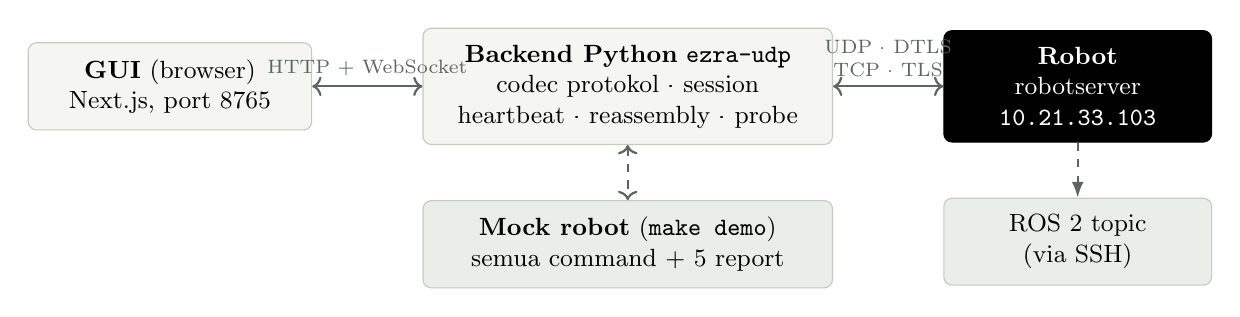
\begin{tikzpicture}[node distance=10mm and 14mm,
  box/.style={draw=ezline,fill=panel,rounded corners=3pt,align=center,inner sep=6pt,font=\small},
  arr/.style={-{Latex[length=2mm]},thick,color=muted}]
  \node[box,minimum width=36mm] (gui) {\textbf{GUI} (browser)\\Next.js, port 8765};
  \node[box,right=of gui,minimum width=52mm] (be) {\textbf{Backend Python} \code{ezra-udp}\\codec protokol · session\\heartbeat · reassembly · probe};
  \node[box,right=of be,minimum width=34mm,fill=black,text=white,draw=black] (robot) {\textbf{Robot}\\robotserver\\\code{10.21.33.103}};
  \node[box,below=7mm of be,minimum width=52mm,fill=well] (mock) {\textbf{Mock robot} (\code{make demo})\\semua command + 5 report};
  \node[box,below=7mm of robot,minimum width=34mm,fill=well] (ros) {ROS 2 topic\\(via SSH)};
  \draw[arr,<->] (gui) -- node[above,font=\scriptsize,text=muted]{HTTP + WebSocket} (be);
  \draw[arr,<->] (be) -- node[above,font=\scriptsize,text=muted,align=center]{UDP · DTLS\\TCP · TLS} (robot);
  \draw[arr,<->,dashed] (be) -- (mock);
  \draw[arr,dashed] (robot) -- (ros);
\end{tikzpicture}
\caption{Satu proses Python menjalankan API, GUI dan (opsional) robot tiruan. Semua offline.}
\end{figure}

\subsection{Kartu saku}

\begin{tabularx}{\linewidth}{@{}L{55mm}Y@{}}
\toprule
\textbf{Perlu apa} & \textbf{Perintah (di folder repo)}\\\midrule
Install (sekali, butuh internet) & \code{make setup}\\
Coba semua fitur tanpa robot & \code{make demo} \ra{} preset \ui{Mock · DTLS} \ra{} \ui{Connect}\\
Cek otomatis semuanya (tanpa robot) & \code{make smoke} \ra{} harus selesai dengan \code{smoke test passed}\\
GUI ke robot & \code{make run} \ra{} \code{http://127.0.0.1:8765}\\
Robot jawab di mode/port mana? & \code{make probe} atau \code{ezra-udp probe -{}-host 10.21.33.103}\\
Uji otomatis dari terminal & \code{ezra-udp suite -t dtls -{}-host 10.21.33.103 -{}-allow-caution}\\
Kirim satu command & \code{ezra-udp send location\_get -t dtls}\\
Lihat report 10 detik & \code{ezra-udp listen -s 10 -t dtls}\\
Decode hex hasil capture & \code{ezra-udp decode "eb 91 eb 90 ..."}\\
Berhenti darurat (GUI) & \ui{Stop} / tombol \code{Esc}; \ui{E-STOP} = stop + soft emergency stop\\
\bottomrule
\end{tabularx}

% ======================================================================
\section{Persiapan sebelum berangkat}\label{sec:prep}

\subsection{Install di Mac}
Butuh Python $\geq$ 3.10 dan Node $\geq$ 20. Python bawaan macOS (\code{/usr/bin/python3}) masih 3.9 --- terlalu
lama; \code{make setup} otomatis memilih \code{python3.14}/\code{3.13}/\ldots{} yang ada di PATH.
\begin{lstlisting}
brew install python@3.13 node            # kalau belum ada
git clone git@github.com:DarmawanRobotics/drds_udp_tools.git
cd drds_udp_tools
make setup                               # .venv + backend + dependensi web
make demo                                # build GUI + server + mock robot, browser terbuka
\end{lstlisting}
\begin{warn}[Lakukan selagi ada internet]
\code{make setup} dan \code{make build} mengunduh paket pip/npm. Setelah itu semuanya jalan offline --- font
GUI ikut dibundel, tidak ada CDN. Di pabrik cukup \code{make serve} atau \code{make run}.
\end{warn}

\subsection{Uji tanpa robot (wajib, 5 menit)}
\begin{enumerate}
\item \code{make demo}, lalu di top bar pilih \ui{Preset \ra{} Mock · DTLS}, tekan \ui{Connect}.
\item Lampu \ui{HB} dan \ui{Reports} hijau, angka HB naik 2 per detik.
\item Tab \ui{Monitor}: kelima panel terisi, rate kira-kira 2/10/2/2/1 Hz.
\item Tab \ui{Test run}: \ui{Probe} ke \code{127.0.0.1} --- DTLS, TLS, UDP 30000 dan TCP 30001 \code{ok}.
\item Centang semua check \emph{safe} + \emph{caution}, \ui{Run} --- semua \code{pass}.
\end{enumerate}
Versi otomatisnya: \code{make smoke}. Perintah ini menjalankan GUI + API + mock robot lalu mengetes keempat
transport, JSON dan XML, heartbeat, dan kelima report dalam $\pm$5 detik. Hasilnya harus \code{smoke test passed}.

Kalau langkah ini lancar, laptop siap; masalah di pabrik berarti ada di jaringan atau konfigurasi robot.

\subsection{Barang bawaan}

\begin{tabularx}{\linewidth}{@{}l Y@{}}
\cb & MacBook + charger, repo sudah \code{make setup} dan GUI sudah di-build\\
\cb & Adapter USB-C ke Ethernet + kabel LAN (bawa cadangan)\\
\cb & Remote robot + akses ke E-stop fisik\\
\cb & PDF protokol V1.0.3 dan manual ini (cetak checklist Bab \ref{sec:checklist})\\
\cb & User/password SSH robot (host locomotion AOS dan navigation NOS)\\
\cb & Sertifikat DTLS/TLS kalau Deep Robotics memberikannya (CA, cert/key klien)\\
\cb & Wireshark (\code{brew install -{}-cask wireshark}) untuk capture bukti\\
\end{tabularx}

\subsection{Pertanyaan untuk tim Deep Robotics / pabrik}
Jawaban ini menentukan mode koneksi dan uji mana yang bisa dijalankan --- tanyakan sebelum mulai.

\begin{tabularx}{\linewidth}{@{}L{62mm}Y@{}}
\toprule
\textbf{Pertanyaan} & \textbf{Kenapa penting}\\\midrule
IP robot (default \code{10.21.33.103}) dan IP host navigasi & semua koneksi + SSH ROS 2\\
Enkripsi aktif? (DTLS 30004 / TLS 30003) & menentukan mode di tool (Bab \ref{sec:modes})\\
Kalau enkripsi dimatikan: port plain berapa? & V1.0.3 tidak menyebutkan; tool menebak 30000/30001\\
Perlu sertifikat klien? CA robot? & handshake ditolak tanpa sertifikat yang benar\\
Unit versi STD atau PRO? & navigasi hanya di PRO (selain itu E00A)\\
SDK mode sudah di-unlock? & tanpa unlock balasannya E007\\
Distro ROS 2 + lokasi workspace \code{drdds} & untuk \code{ros2 topic echo} (Lampiran \ref{app:ros2})\\
Nilai state ``RL control'' untuk \code{/MOTION\_STATE} & diagram state tidak ter-render di PDF\\
Ada peta + docking station untuk uji navigasi/charging? & uji Tahap 10 butuh keduanya\\
\bottomrule
\end{tabularx}

% ======================================================================
\section{Mode koneksi: UDP, DTLS, TCP, TLS}\label{sec:modes}

Isi pesannya \textbf{sama persis} di keempat mode: header 16 byte + ASDU JSON/XML (Bab \ref{sec:protocol}).
Yang berbeda adalah \emph{cara mengangkutnya}: lewat datagram atau aliran byte, terenkripsi atau tidak,
dan apa yang terjadi kalau paket hilang.

\begin{figure}[htbp]
\centering
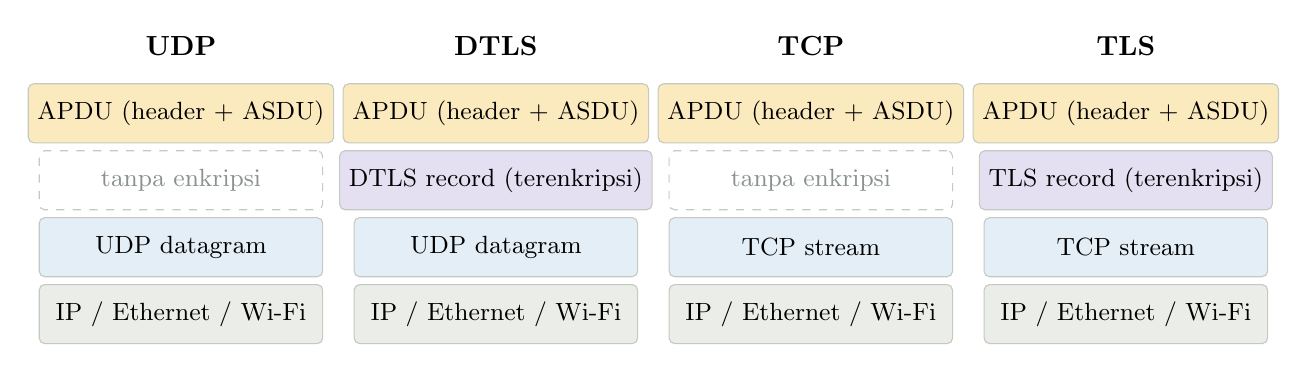
\begin{tikzpicture}[x=40mm,y=8.5mm,
  lay/.style={draw=ezline,rounded corners=2pt,minimum width=36mm,minimum height=7.5mm,font=\small,align=center},
  apdu/.style={lay,fill=signal!25},enc/.style={lay,fill=bid!18},tr/.style={lay,fill=tx!12},ip/.style={lay,fill=well}]
  \foreach \xx/\nm/\en/\tp in {0/UDP/0/UDP datagram,1/DTLS/1/UDP datagram,2/TCP/0/TCP stream,3/TLS/1/TCP stream} {
    \node[font=\bfseries] at (\xx,4.1) {\nm};
    \node[apdu] at (\xx,3.1) {APDU (header + ASDU)};
    \ifnum\en=1 \node[enc] at (\xx,2.1) {\nm\ record (terenkripsi)}; \else \node[lay,draw=ezline,dashed,text=faint] at (\xx,2.1) {tanpa enkripsi}; \fi
    \node[tr] at (\xx,1.1) {\tp};
    \node[ip] at (\xx,0.1) {IP / Ethernet / Wi-Fi};
  }
\end{tikzpicture}
\caption{Lapisan tiap mode. Kotak kuning sama di semua mode --- itulah yang di-decode tool.}
\end{figure}

\subsection{Perbandingan cepat}
\begin{xltabular}{\linewidth}{@{}L{31mm}YYYY@{}}
\toprule
 & \textbf{UDP (plain)} & \textbf{DTLS} & \textbf{TCP (plain)} & \textbf{TLS}\\\midrule
\endhead
Port robot & 30000\textsuperscript{*} & \textbf{30004} (default) & 30001\textsuperscript{*} & \textbf{30003} (default)\\
Enkripsi & tidak & ya (DTLS 1.2) & tidak & ya (TLS 1.2/1.3)\\
Koneksi & tanpa koneksi & sesi DTLS di atas UDP & koneksi TCP & koneksi TCP + sesi TLS\\
Handshake & tidak ada & ClientHello, cookie, sertifikat & 3-way TCP & TCP + handshake TLS\\
Batas pesan & 1 datagram = 1 APDU & 1 record = 1 APDU & aliran byte; dipotong lewat sync \code{EB 91 EB 90} + length & sama dengan TCP\\
Paket hilang & hilang begitu saja & hilang; handshake diulang otomatis & dikirim ulang, urutan dijamin & sama dengan TCP\\
Efek ke stream axis 10--20 Hz & paling mulus & mulus & bisa tersendat saat retransmit & bisa tersendat\\
Port salah/tertutup & ICMP \emph{port unreachable} & handshake timeout / ICMP & \emph{connection refused} & refused / handshake error\\
Isi di Wireshark & terbaca & terenkripsi & terbaca & terenkripsi\\
Pakai kapan & enkripsi dimatikan; debug isi paket & \textbf{default robot} & jaringan yang membuang UDP & fallback terenkripsi kalau DTLS bermasalah\\
\bottomrule
\end{xltabular}
{\small\textsuperscript{*} Port plain tidak disebut di V1.0.3. Nilai ini diambil dari dokumen Deep Robotics versi lama; \code{probe}
juga mencoba 30004/30003 tanpa enkripsi.}

\subsection{UDP (plain)}
Setiap APDU dikirim sebagai satu datagram UDP; tidak ada koneksi maupun handshake. Tool mengirim heartbeat,
command dan menerima balasan + report lewat \textbf{satu socket}, sehingga robot tahu ke IP:port mana report
harus dikirim (robot mengirim report ke pengirim heartbeat).
\begin{itemize}
\item \textbf{Kelebihan:} paling sederhana, latensi terendah, isi paket bisa langsung dibaca di Wireshark
      (filter \code{udp.port == 30000}).
\item \textbf{Kekurangan:} tidak terenkripsi; paket bisa hilang tanpa pemberitahuan. Sesekali satu report hilang
      itu wajar --- yang tidak wajar kalau rate jauh di bawah spesifikasi.
\item \textbf{Di tool:} socket dibuat ``connected'' secara default. Kalau port tujuan tertutup, OS mengembalikan
      ICMP \emph{port unreachable} dan tool menampilkannya di log. Kalau robot ternyata membalas dari port lain,
      matikan \ui{Connected UDP socket} di settings.
\end{itemize}

\subsection{DTLS --- UDP terenkripsi (default robot, port 30004)}
DTLS adalah TLS yang disesuaikan untuk datagram. Sebelum data mengalir, klien dan robot melakukan handshake;
setelah itu tiap APDU dibungkus dalam satu \emph{record} terenkripsi (misalnya AES-GCM) di dalam satu datagram UDP.

\begin{figure}[htbp]
\centering
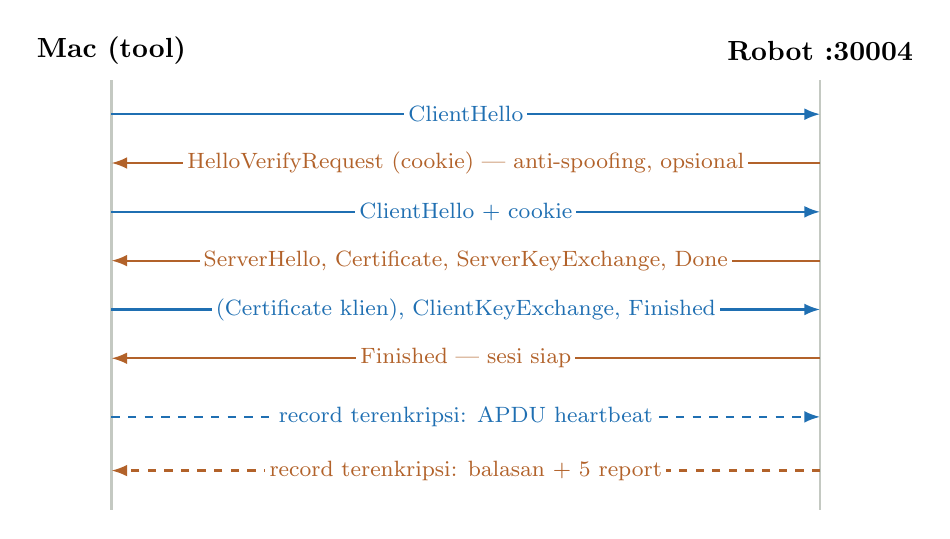
\begin{tikzpicture}[y=-6.2mm,font=\small,
  msg/.style={-{Latex[length=2mm]},thick},lbl/.style={fill=white,inner sep=1.5pt,font=\footnotesize}]
  \node[font=\bfseries] at (0,0) {Mac (tool)};
  \node[font=\bfseries] at (9,0) {Robot :30004};
  \draw[ezline,thick] (0,0.6) -- (0,9.4); \draw[ezline,thick] (9,0.6) -- (9,9.4);
  \draw[msg,tx] (0,1.3) -- node[lbl]{ClientHello} (9,1.3);
  \draw[msg,rx] (9,2.3) -- node[lbl]{HelloVerifyRequest (cookie) --- anti-spoofing, opsional} (0,2.3);
  \draw[msg,tx] (0,3.3) -- node[lbl]{ClientHello + cookie} (9,3.3);
  \draw[msg,rx] (9,4.3) -- node[lbl]{ServerHello, Certificate, ServerKeyExchange, Done} (0,4.3);
  \draw[msg,tx] (0,5.3) -- node[lbl]{(Certificate klien), ClientKeyExchange, Finished} (9,5.3);
  \draw[msg,rx] (9,6.3) -- node[lbl]{Finished --- sesi siap} (0,6.3);
  \draw[msg,tx,dashed] (0,7.5) -- node[lbl]{record terenkripsi: APDU heartbeat} (9,7.5);
  \draw[msg,rx,dashed] (9,8.6) -- node[lbl]{record terenkripsi: balasan + 5 report} (0,8.6);
\end{tikzpicture}
\caption{Handshake DTLS 1.2. Paket handshake yang hilang dikirim ulang otomatis lewat timer.}
\end{figure}

\begin{itemize}
\item \textbf{Record harus muat satu datagram.} Tool memakai MTU 1400 byte; APDU maksimal 1016 byte
      (16 header + 1000 ASDU), jadi aman.
\item \textbf{Sesi terikat ke IP:port kedua sisi.} Kalau robot reboot atau sesinya direset, record dari sesi lama
      diabaikan diam-diam. Gejalanya: top bar merah \ui{Link lost}. Solusinya: \ui{Disconnect} \ra{} \ui{Connect}.
\item \textbf{Wireshark} hanya melihat handshake dan record terenkripsi. Isi APDU yang sudah didekripsi ada di tab
      \ui{Traffic} --- di situlah bukti isinya.
\item \textbf{Di tool:} OpenSSL 3 lewat pyOpenSSL. Verifikasi sertifikat \emph{mati} secara default karena sertifikat
      robot biasanya self-signed. CA, sertifikat/kunci klien (mutual TLS), SNI, cipher, MTU dan \ui{Compat mode}
      bisa diatur di settings.
\end{itemize}

\subsection{TCP (plain)}
Satu koneksi TCP; datanya berupa aliran byte tanpa batas pesan. Tool memotong APDU dengan mencari sync
\code{EB 91 EB 90} lalu membaca field \emph{length}. Kalau ada byte sampah, tool resync otomatis dan
mencatatnya di log.
\begin{itemize}
\item \textbf{Terjamin sampai dan berurutan}, tapi paket yang hilang dikirim ulang dan menahan paket
      sesudahnya (\emph{head-of-line blocking}). Untuk teleop 10--20 Hz, UDP/DTLS lebih mulus.
\item Port tertutup langsung ketahuan: \emph{connection refused}.
\item Kalau TCP plain dikirim ke port TLS (30003), robot menutup koneksi tanpa membalas. Tool memberi petunjuk:
      ``\emph{port probably expects TLS}''.
\end{itemize}

\subsection{TLS --- TCP terenkripsi (default robot, port 30003)}
TCP ditambah handshake TLS (biasanya TLS 1.2 atau 1.3); setelah itu perilakunya sama seperti TCP, hanya
terenkripsi. Ini \textbf{fallback terbaik} kalau DTLS diblok di jaringan atau handshake DTLS bermasalah.
Opsinya sama dengan DTLS: verify, CA, sertifikat klien, SNI, cipher, compat.

\subsection{Port dan enkripsi di robot}
\begin{itemize}
\item Menurut PDF: \emph{``Port communication is encrypted by default''}. Di \code{10.21.33.103} yang terbuka adalah
      DTLS port \code{30004} dan TLS port \code{30003}.
\item Enkripsi bisa dimatikan dengan mengubah file konfigurasi \code{robotserver} (minta bantuan technical support
      Deep Robotics). File itu tidak ditimpa saat system update.
\item Setelah enkripsi dimatikan, port plain tidak disebutkan di V1.0.3. Gunakan \code{probe} untuk mencari tahu.
\end{itemize}

\subsection{Memilih mode: probe dulu}\label{sec:choose}
Jangan menebak. \ui{Test run \ra{} Probe} di GUI (atau \code{make probe}) mengirim satu heartbeat lewat enam
kombinasi --- DTLS 30004, TLS 30003, UDP 30000, UDP 30004, TCP 30001, TCP 30003 --- masing-masing dari socket
sendiri, lalu menampilkan hasilnya. Tombol \ui{Use} langsung mengisi mode + port ke top bar.

\begin{figure}[htbp]
\centering
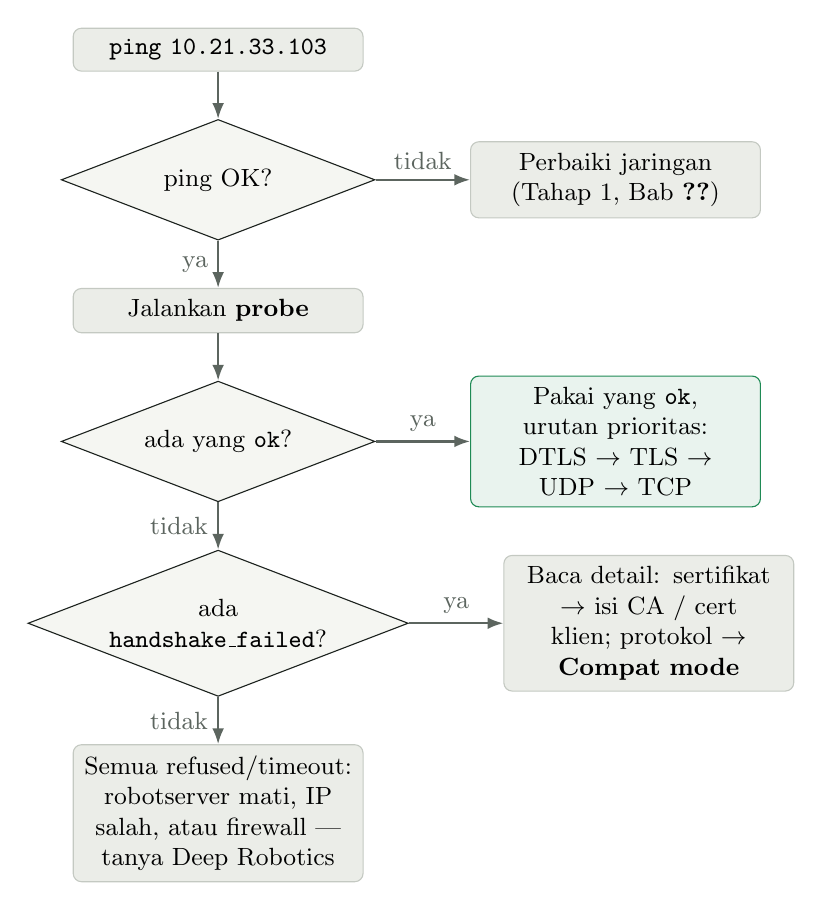
\begin{tikzpicture}[node distance=6mm and 8mm,font=\small,
  q/.style={draw=ink,fill=panel,diamond,aspect=2.6,inner sep=1pt,align=center,text width=30mm},
  a/.style={draw=ezline,fill=well,rounded corners=3pt,align=center,text width=34mm,inner sep=4pt},
  g/.style={draw=lamp,fill=lamp!10,rounded corners=3pt,align=center,text width=34mm,inner sep=4pt},
  arr/.style={-{Latex[length=2mm]},thick,color=muted}]
  \node[a] (ping) {\code{ping 10.21.33.103}};
  \node[q,below=of ping] (pok) {ping OK?};
  \node[a,right=12mm of pok] (net) {Perbaiki jaringan\\(Tahap 1, Bab \ref{sec:trouble})};
  \node[a,below=of pok] (probe) {Jalankan \textbf{probe}};
  \node[q,below=of probe] (any) {ada yang \code{ok}?};
  \node[g,right=12mm of any] (use) {Pakai yang \code{ok}, urutan prioritas:\\DTLS \ra{} TLS \ra{} UDP \ra{} TCP};
  \node[q,below=of any] (hs) {ada \code{handshake\_failed}?};
  \node[a,right=12mm of hs] (cert) {Baca detail: sertifikat \ra{} isi CA / cert klien; protokol \ra{} \ui{Compat mode}};
  \node[a,below=of hs] (none) {Semua refused/timeout: robotserver mati, IP salah, atau firewall --- tanya Deep Robotics};
  \draw[arr] (ping) -- (pok); \draw[arr] (pok) -- node[above]{tidak} (net);
  \draw[arr] (pok) -- node[left]{ya} (probe); \draw[arr] (probe) -- (any);
  \draw[arr] (any) -- node[above]{ya} (use); \draw[arr] (any) -- node[left]{tidak} (hs);
  \draw[arr] (hs) -- node[above]{ya} (cert); \draw[arr] (hs) -- node[left]{tidak} (none);
\end{tikzpicture}
\caption{Alur memilih mode koneksi.}
\end{figure}

\begin{xltabular}{\linewidth}{@{}L{30mm}YY@{}}
\toprule
\textbf{Hasil probe} & \textbf{Artinya} & \textbf{Lakukan}\\\midrule
\endhead
\code{ok} & heartbeat dibalas --- jalur ini bekerja & klik \ui{Use}, lalu \ui{Connect}\\
\code{no\_reply} & terkirim, tapi tidak ada balasan & mode salah untuk port ini (mis. UDP plain ke port DTLS), atau robot membalas dari port lain\\
\code{refused} & ICMP port unreachable / TCP RST & tidak ada yang mendengar di port itu\\
\code{unreachable} & tidak ada rute ke robot & Mac belum di subnet robot / IP salah (Tahap 1)\\
\code{handshake\_failed} & DTLS/TLS ditolak & ikuti petunjuk di detail: sertifikat, plain port, atau compat mode\\
\code{timeout} & tidak ada jawaban sama sekali & firewall, robotserver belum jalan, atau jaringan putus\\
\bottomrule
\end{xltabular}

\subsection{Opsi keamanan (settings \gear)}
\begin{xltabular}{\linewidth}{@{}L{42mm}Y@{}}
\toprule
\textbf{Opsi} & \textbf{Pakai kalau}\\\midrule
\endhead
Verify certificate & ingin memastikan identitas robot; isi juga \emph{CA file}. Default mati (self-signed).\\
CA file & Deep Robotics memberi sertifikat CA robot (\code{.pem}).\\
Client certificate + key & robot meminta mutual TLS; error-nya menyebut \emph{certificate required}.\\
Server name (SNI) & sertifikat robot memakai nama host tertentu (jarang dibutuhkan untuk alamat IP).\\
Cipher list & ingin memaksa cipher tertentu (sintaks OpenSSL).\\
\textbf{Compat mode} & error \emph{protocol version}, \emph{no ciphers} atau \emph{handshake failure}: mengizinkan TLS/DTLS versi lama dan cipher lemah (\code{DEFAULT:@SECLEVEL=0}). Matikan lagi setelah selesai.\\
DTLS MTU & jaringan dengan MTU kecil (VPN/tunnel); turunkan ke 1200.\\
Local port & robot hanya menerima dari port tertentu; 0 = acak.\\
\bottomrule
\end{xltabular}

\subsection{JSON atau XML}
Byte ke-8 header menyatakan format ASDU: \code{0x01} JSON, \code{0x00} XML. Dokumen merekomendasikan JSON
(lebih cepat, struktur lebih lengkap). Toggle \ui{JSON / XML} di top bar mengubah format semua request.
Uji XML minimal sekali (ada di conformance run) untuk memastikan robot mendukungnya.

% ======================================================================
\section{Protokol singkat}\label{sec:protocol}

\subsection{Header APDU (16 byte, little endian)}
\begin{center}\ribbon{0.95}\end{center}

\begin{tabularx}{\linewidth}{@{}L{14mm}L{10mm}L{30mm}Y@{}}
\toprule
\textbf{Offset} & \textbf{Size} & \textbf{Field} & \textbf{Isi}\\\midrule
0 & 4 & sync & tetap \code{EB 91 EB 90}\\
4 & 2 & length & jumlah byte ASDU (maks 1000 per frame)\\
6 & 2 & message id & 0--65535 lalu kembali ke 0; balasan memakai id yang sama\\
8 & 1 & ASDU format & \code{0x00} XML, \code{0x01} JSON\\
9 & 1 & packet sequence & 0--255, untuk pesan yang dipecah (multi-packet)\\
10 & 1 & protocol version & tetap 1\\
11 & 5 & reserved & nol\\
\bottomrule
\end{tabularx}

\subsection{ASDU}
\begin{lstlisting}
{"PatrolDevice": {"Type": 1048676, "Command": 5,
                  "Time": "2026-01-01 00:00:00.000", "Items": {}}}
\end{lstlisting}
\code{Type} + \code{Command} menentukan jenis pesan, \code{Time} berisi waktu lokal, \code{Items} berisi parameter.
Di XML, list menjadi elemen berulang (\code{<Led>...</Led><Led>...</Led>}).

\subsection{Request, balasan, dan message id}
\begin{itemize}
\item Setiap request mendapat \textbf{balasan status} (\S1.5): \code{ErrorCode} + \code{ErrorMessage}; 0 = Success.
\item Query (\S1.4.2, 1.4.3, 1.4.5, 1.4.6) membalas dengan \textbf{data}.
\item \textbf{Axis} (\S1.2.5) dan \textbf{velocity} (\S1.2.6) \emph{tidak punya balasan}; di GUI tertulis ``no reply''.
\item \textbf{Navigation task} (\S1.4.4): balasan status langsung, lalu \textbf{balasan hasil} saat tugas selesai,
      gagal, atau dibatalkan. Tool tetap mendengarkan sampai 30 menit; balasan susulan muncul di \ui{Timeline}.
\item Heartbeat juga memakai message id, jadi nomor id melompat-lompat --- itu normal.
\end{itemize}

\subsection{Heartbeat dan 5 status report}
Robot mengirim report ke IP:port yang \textbf{terus} mengirim heartbeat ($\geq$ 1 Hz; tool memakai 2 Hz).
Kalau 2 detik tidak ada heartbeat, report berhenti dan koneksi harus dibangun ulang.

\begin{tabularx}{\linewidth}{@{}L{13mm}L{27mm}L{23mm}L{24mm}Y@{}}
\toprule
\textbf{\S} & \textbf{Report} & \textbf{Type} & \textbf{Rate} & \textbf{Isi utama}\\\midrule
1.3.1.1 & Basic Status & \code{0x0010 0064} & 2 Hz & motion state, gait, HES, mode, sleep, model/versi, charge\\
1.3.1.2 & Motion Control & \code{0x0010 0001} & 10 Hz & IMU, kecepatan, tinggi, 16 sudut joint\\
1.3.1.3 & Device State & \code{0x0010 0002} & 2 Hz & baterai, suhu motor/driver, GPS, lidar/video, CPU\\
1.3.1.4 & Abnormal Status & \code{0x0010 007F} & 2 Hz + saat berubah & daftar fault aktif\\
1.3.1.5 & Navigation Status & \code{0x0010 0003} & 1 Hz & status tugas navigasi + pose di peta\\
\bottomrule
\end{tabularx}

Semua report memakai Command \code{0x00F0 0000}. Device State ($\pm$1,8 KB) biasanya datang sebagai 2 paket
(multi-packet); tool menggabungkannya dan menampilkan ``2 packets''.

% ======================================================================
\section{Panduan GUI}\label{sec:gui}

\subsection{Top bar}
\begin{figure}[htbp]
\centering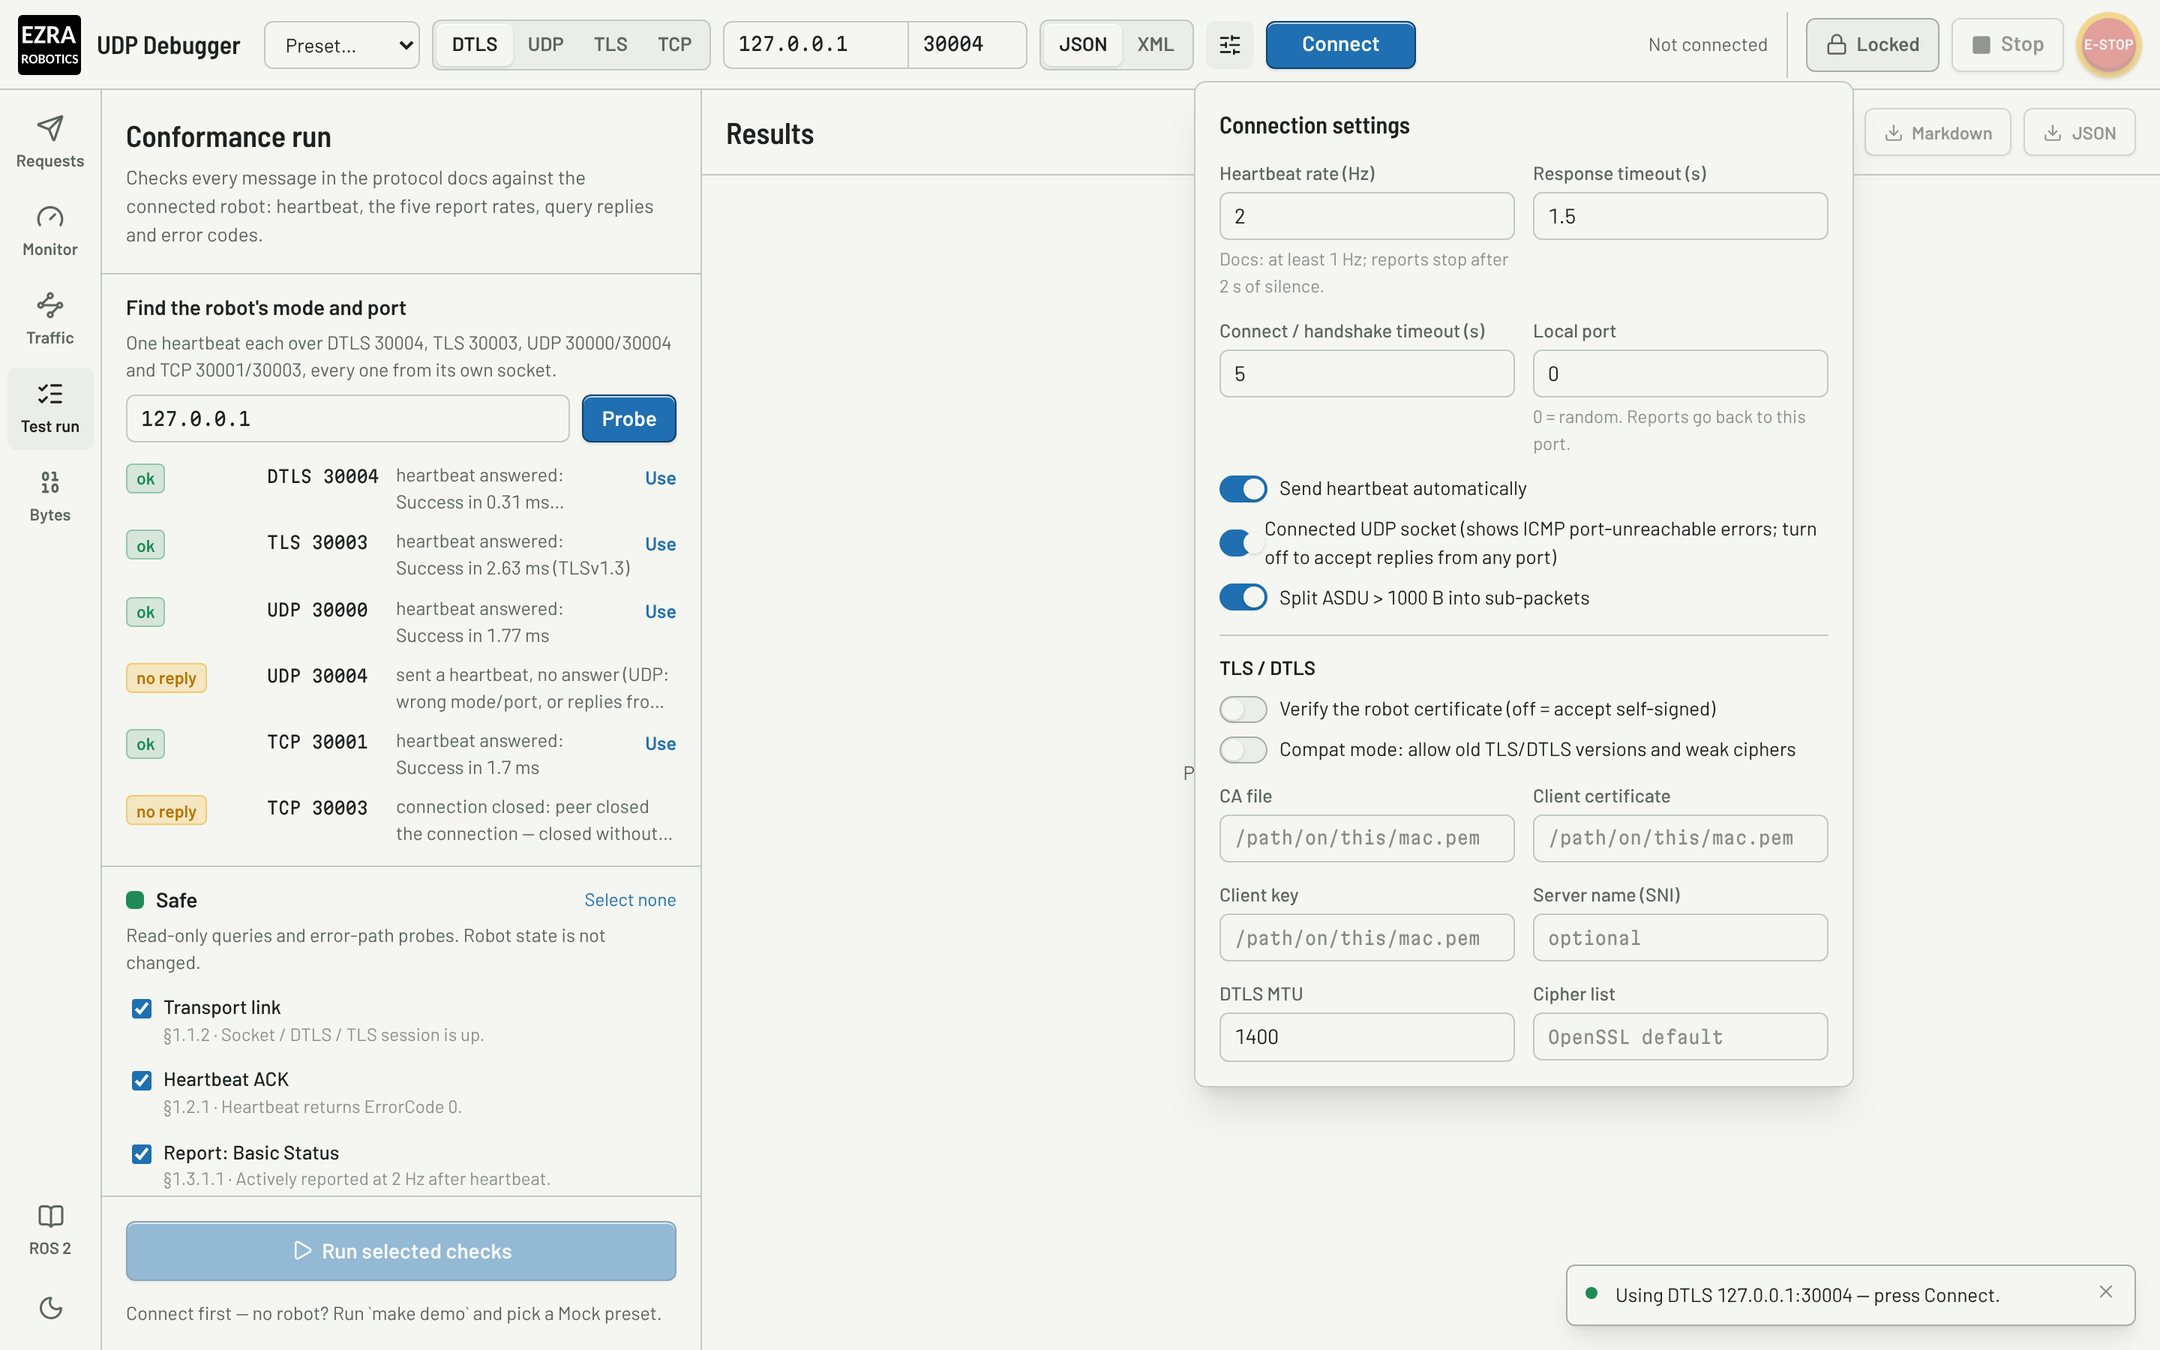
\includegraphics[width=\linewidth]{figures/gui-settings.jpg}
\caption{Top bar dengan settings koneksi terbuka.}
\end{figure}
\begin{itemize}
\item \ui{Preset} --- target siap pakai: Robot DTLS/TLS/UDP/TCP dan Mock.
\item \ui{DTLS / UDP / TLS / TCP}, host, port, dan \ui{JSON / XML}.
\item \gear{} settings: rate heartbeat, timeout, local port, connected UDP socket, split ASDU, dan semua opsi TLS/DTLS (Bab \ref{sec:modes}).
\item Lampu \ui{HB} (acked/sent, berkedip setiap ACK) dan \ui{Reports} (hijau kalau ada report dalam 2,5 detik terakhir).
      Kalau ACK berhenti 3 detik, keduanya diganti tulisan merah \ui{Link lost}.
\item \ui{Locked / Armed} --- command yang menggerakkan robot diblok sampai \ui{Armed}. Setiap halaman dibuka
      selalu mulai \ui{Locked}.
\item \ui{Stop} (atau \code{Esc}): menghentikan semua stream, mengirim axis 0 + velocity 0, dan membatalkan navigasi.
\item \ui{E-STOP}: \ui{Stop} lalu \code{MotionParam = -2} (soft emergency stop / joint damping). Robot akan lemas dan duduk.
\end{itemize}

\subsection{Requests}
\begin{figure}[htbp]
\centering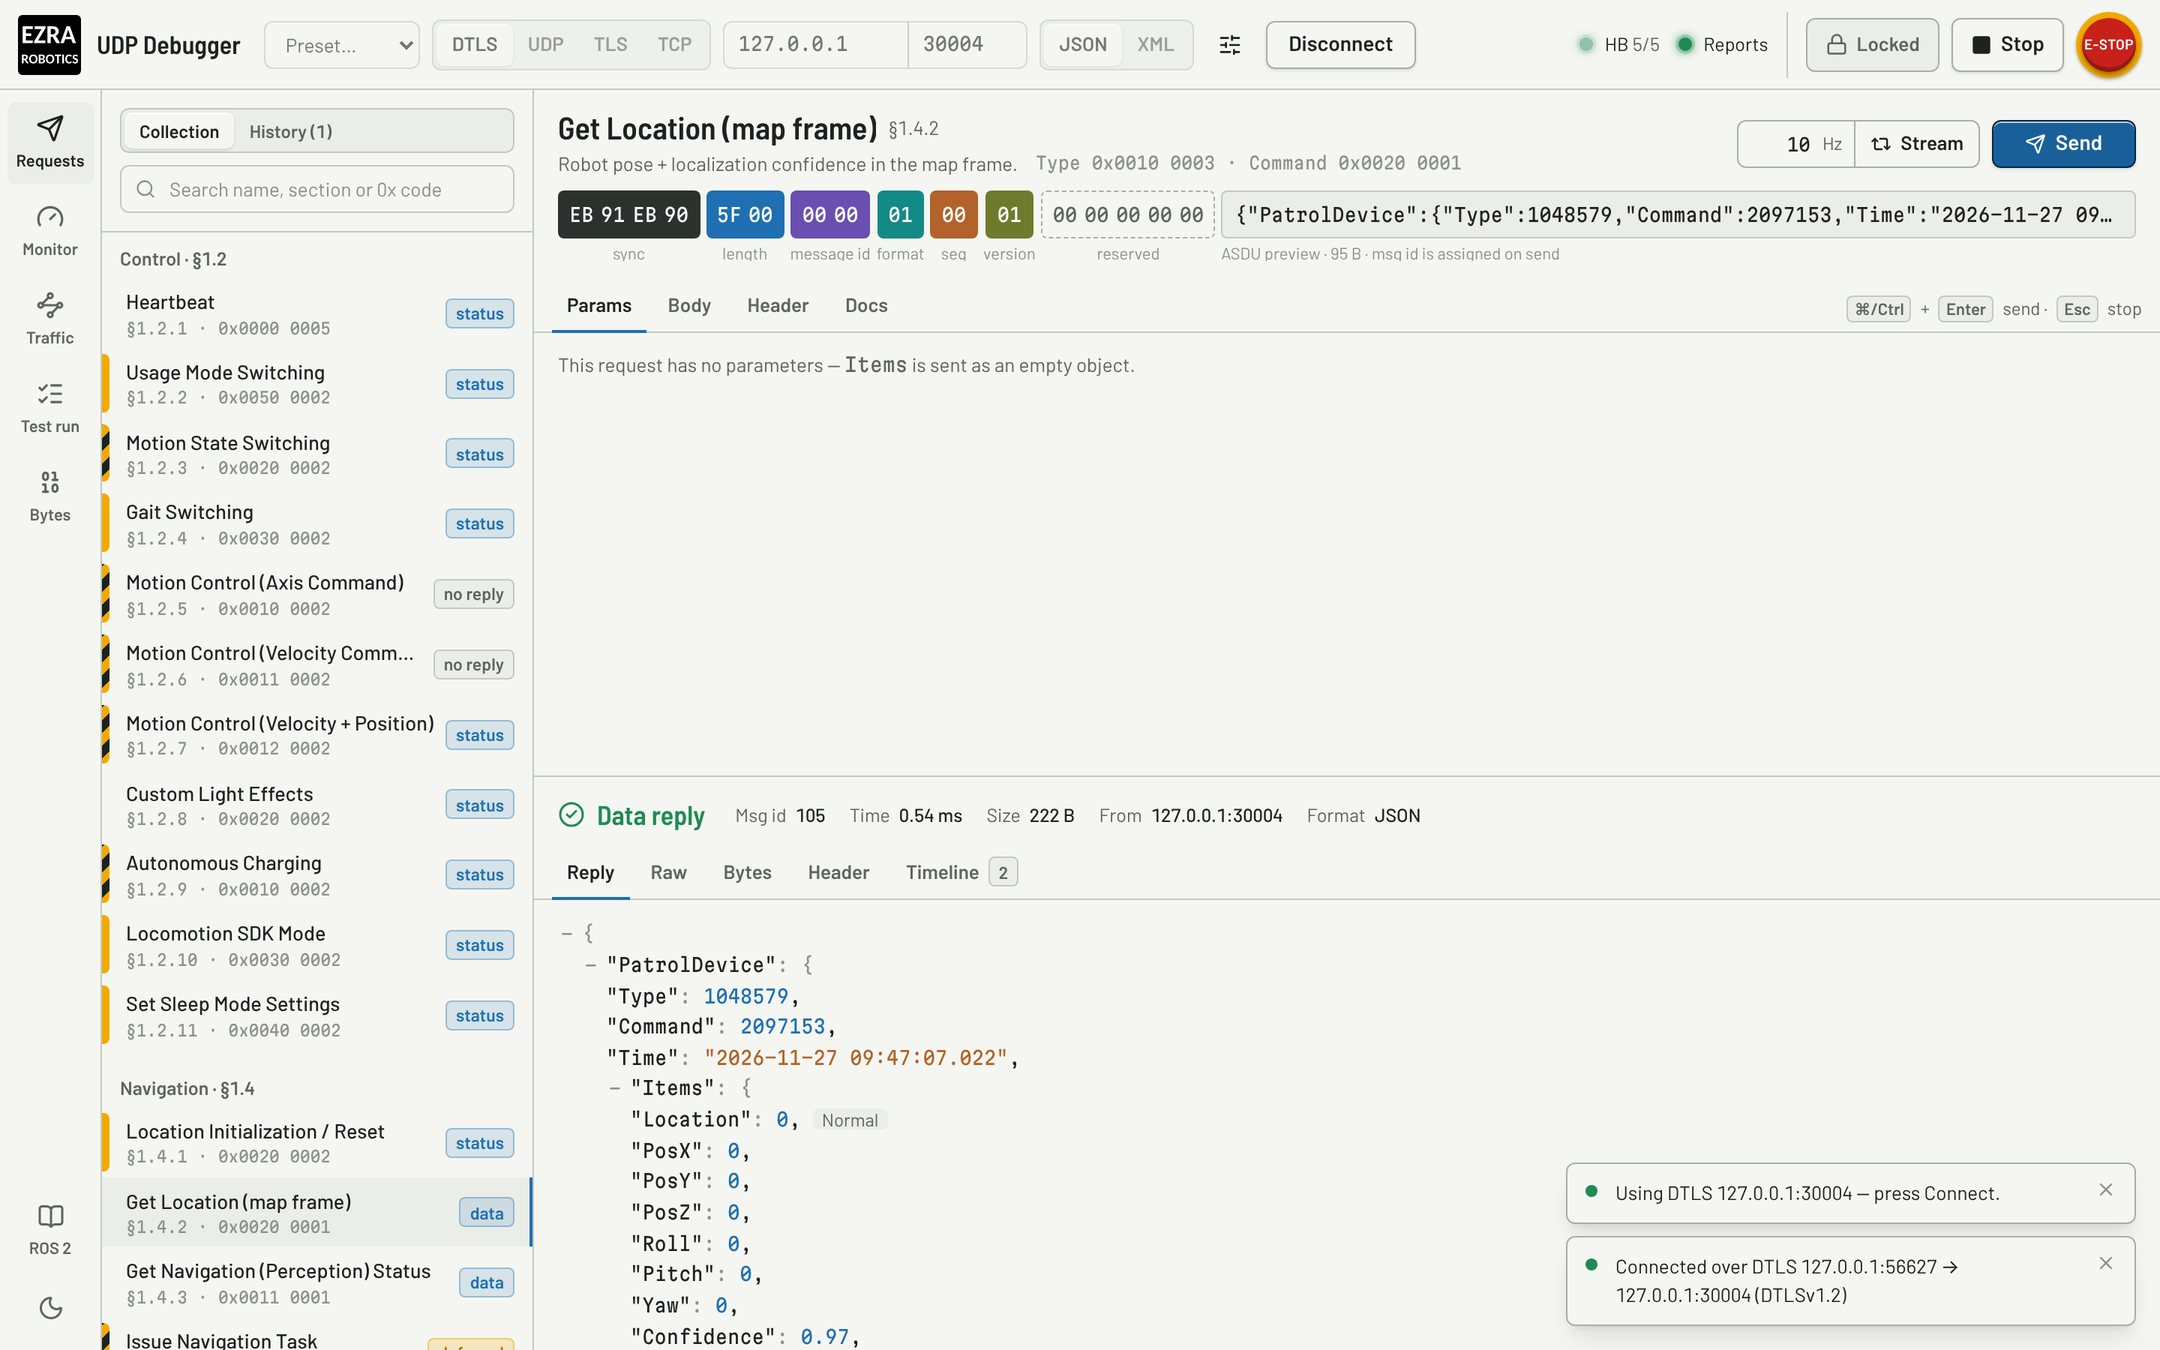
\includegraphics[width=\linewidth]{figures/gui-requests.jpg}
\caption{Requests: koleksi command, form parameter, byte ribbon, dan balasan robot.}
\end{figure}
\begin{itemize}
\item Sidebar berisi semua command \S1.2 dan \S1.4. Garis \textbf{hazard kuning-hitam} = menggerakkan robot;
      kuning polos = mengubah state. Chip \code{status}/\code{data}/\code{no reply}/\code{deferred} menunjukkan jenis balasan.
\item Byte ribbon memperlihatkan 16 byte header + ASDU yang akan dikirim, dan ikut berubah saat parameter diedit.
\item Tab \ui{Params} (form dari dokumen), \ui{Body} (mode raw: teks dikirim apa adanya --- untuk uji E002),
      \ui{Header} (override msg id/format/version/length/sync untuk uji frame yang salah), \ui{Docs}.
\item \ui{Send} (\code{Cmd/Ctrl+Enter}), \ui{Stream} N Hz, dan \ui{Hold to move} untuk axis/velocity: selama ditekan
      tool mengirim terus, saat dilepas tool mengirim nol (\emph{dead-man switch}).
\item Panel balasan: kode + label (mis. \code{0xE003 Unsupported protocol type}), waktu, ukuran, msg id, alamat
      pengirim. Tab \ui{Reply} memberi label enum otomatis (mis. \code{"MotionState": 1} \ra{} Stand), lalu ada
      \ui{Raw}, \ui{Bytes}, \ui{Header}, dan \ui{Timeline} (termasuk balasan susulan).
\item \ui{Custom message}: Type/Command apa saja --- untuk menguji pesan di luar dokumen.
\item \ui{History}: request yang pernah dikirim; klik untuk memuat ulang.
\end{itemize}

\subsection{Monitor}
\begin{figure}[htbp]
\centering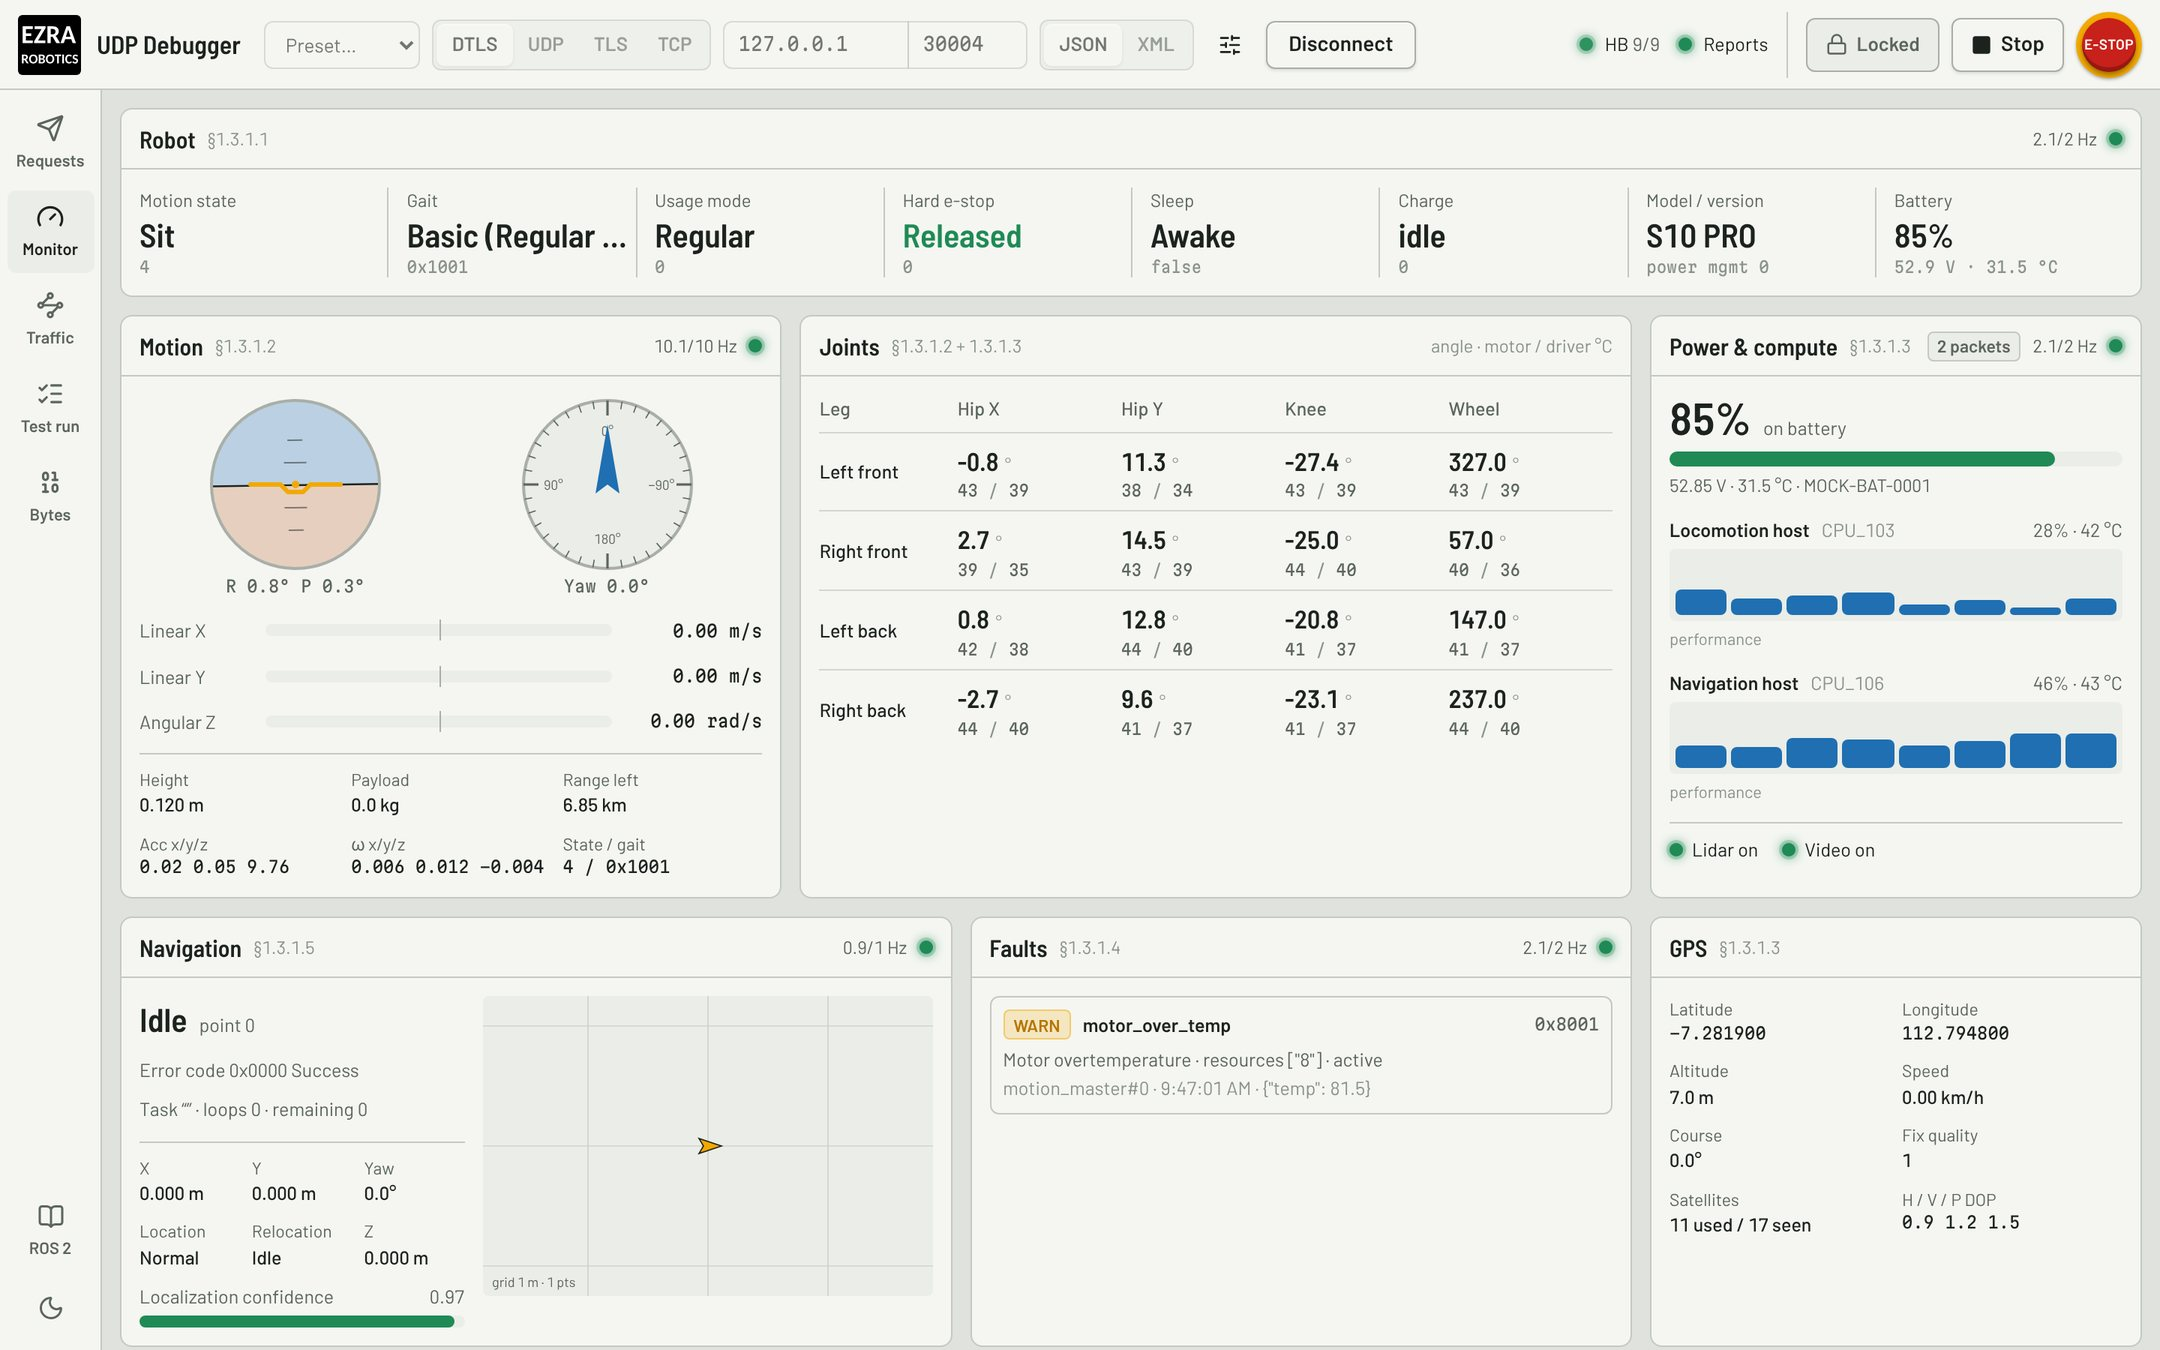
\includegraphics[width=\linewidth]{figures/gui-monitor.jpg}
\caption{Monitor: instrumen untuk kelima report.}
\end{figure}
Setiap panel menampilkan rate terukur dibanding rate di dokumen (mis. \code{9.8/10 Hz}) dan lampu kesegaran data.
Panelnya: robot (state, gait, mode, HES, sleep, charge, model, baterai), motion (horizon roll/pitch, heading,
kecepatan, IMU), joints (16 sudut + suhu motor/driver), power \& compute (baterai, CPU per core untuk host
locomotion dan navigation, lidar/video), navigation (status tugas, pose, confidence, jejak pose), faults, dan GPS.

\subsection{Traffic}
\begin{figure}[htbp]
\centering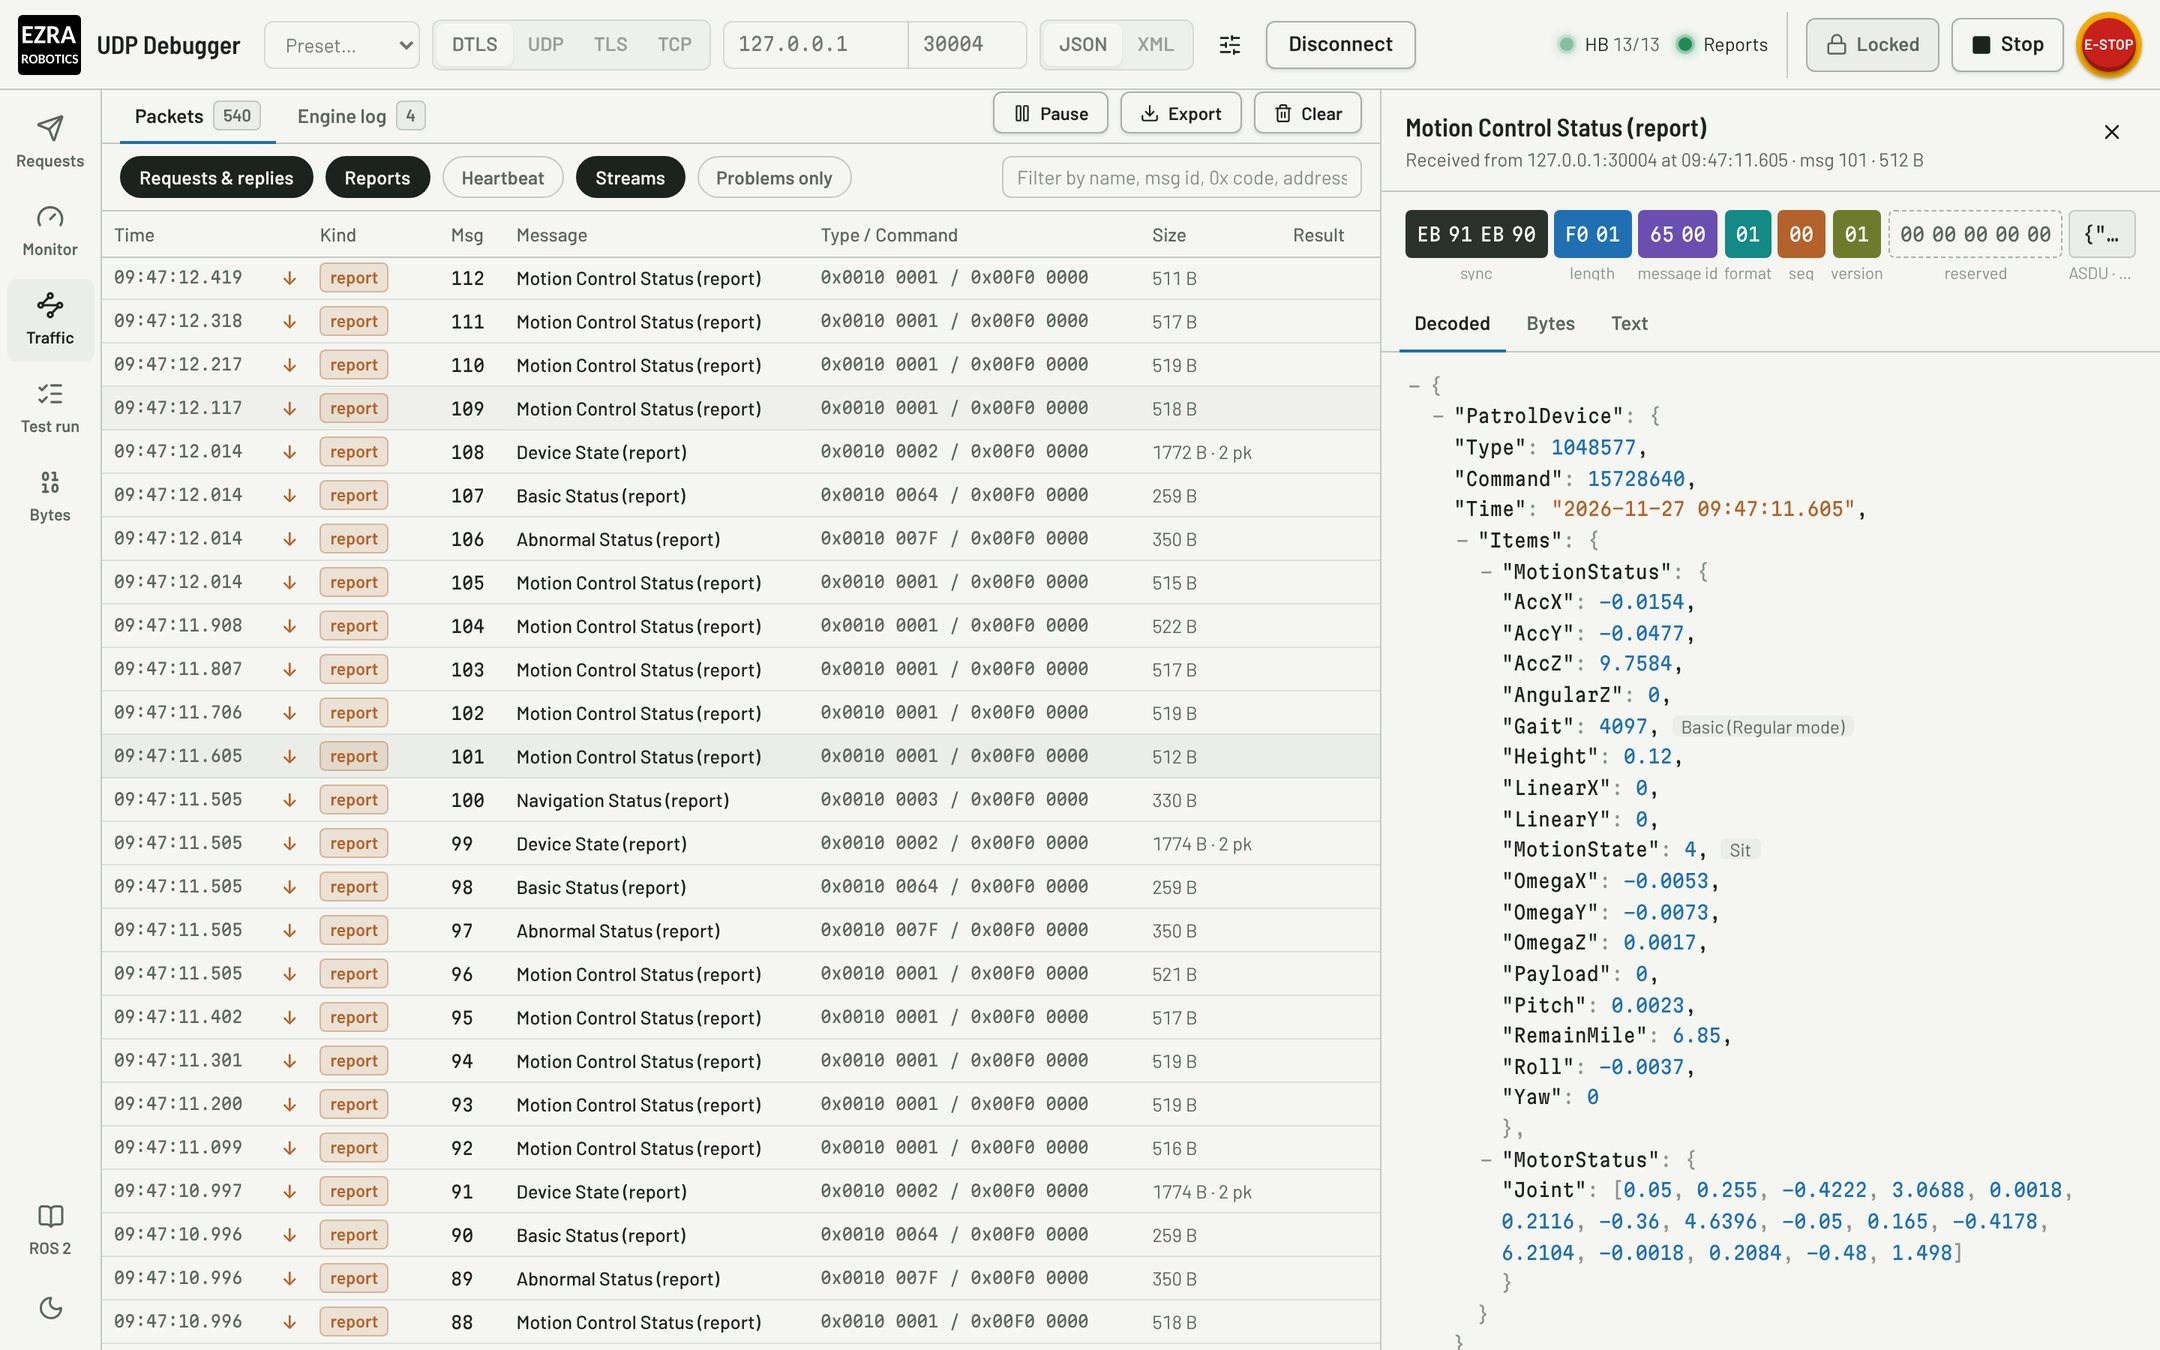
\includegraphics[width=\linewidth]{figures/gui-traffic.jpg}
\caption{Traffic: semua paket masuk/keluar, detail byte dan JSON.}
\end{figure}
Filter \ui{Requests \& replies}, \ui{Reports}, \ui{Heartbeat}, \ui{Streams}, dan \ui{Problems only}. \ui{Pause}
membekukan tampilan, \ui{Export} menyimpan JSON (bukti untuk dibawa pulang). Tab \ui{Engine log} mencatat handshake,
ICMP error, \emph{link lost/restored}, dan perubahan fault (START/STOP).

\subsection{Test run dan Probe}
\begin{figure}[htbp]
\centering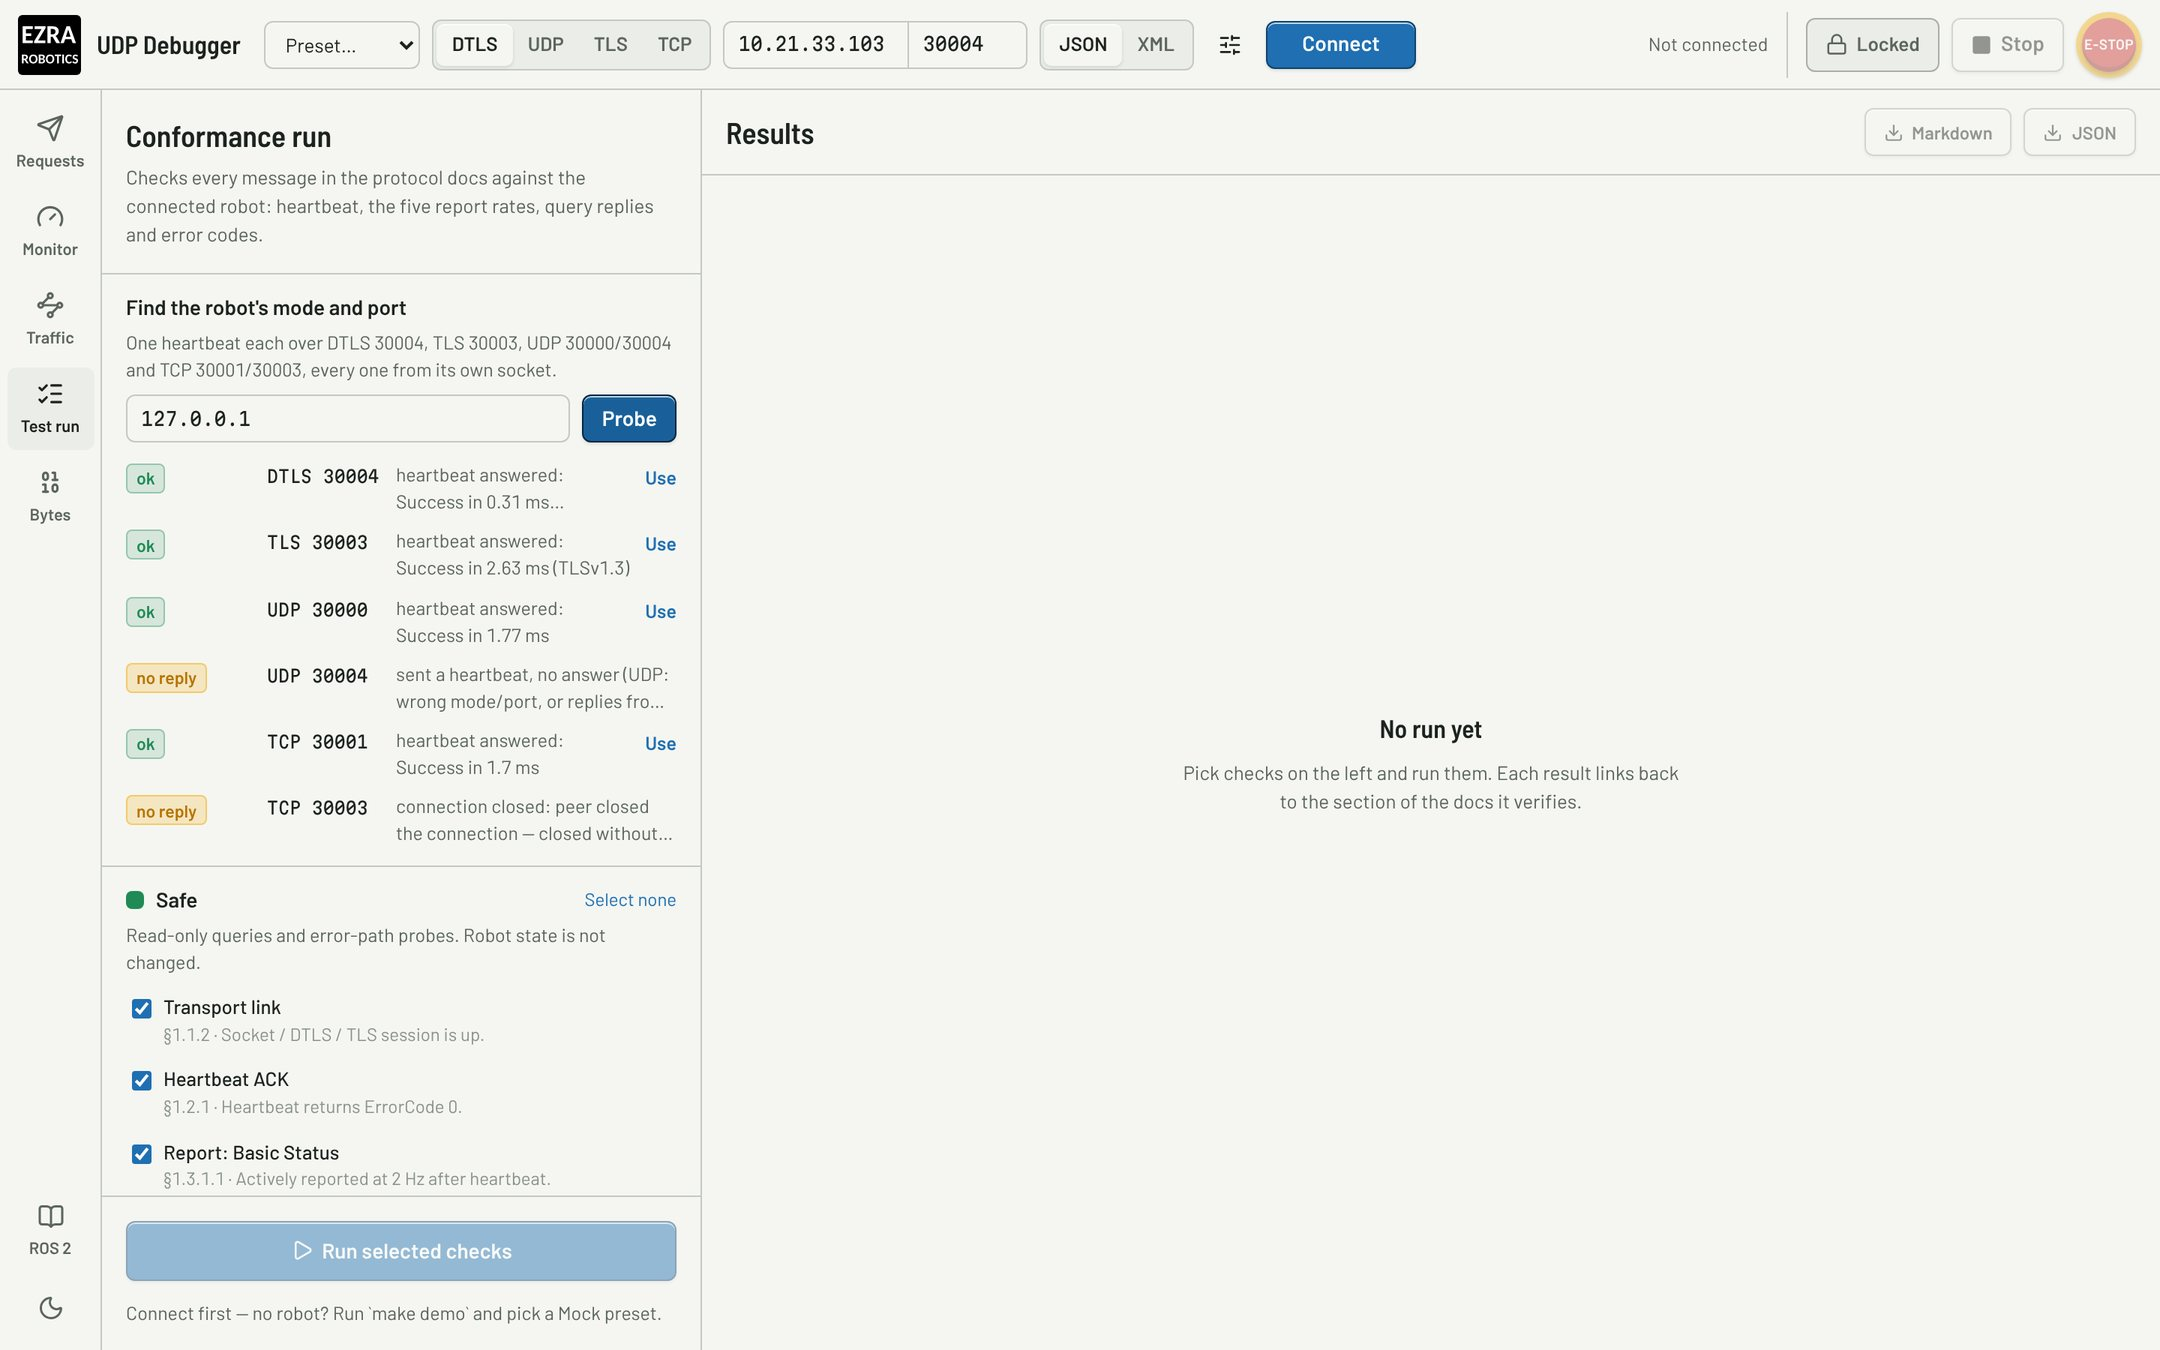
\includegraphics[width=\linewidth]{figures/gui-probe.jpg}
\caption{Probe: mencari mode/port yang dijawab robot (di sini ke mock robot).}
\end{figure}
\begin{figure}[htbp]
\centering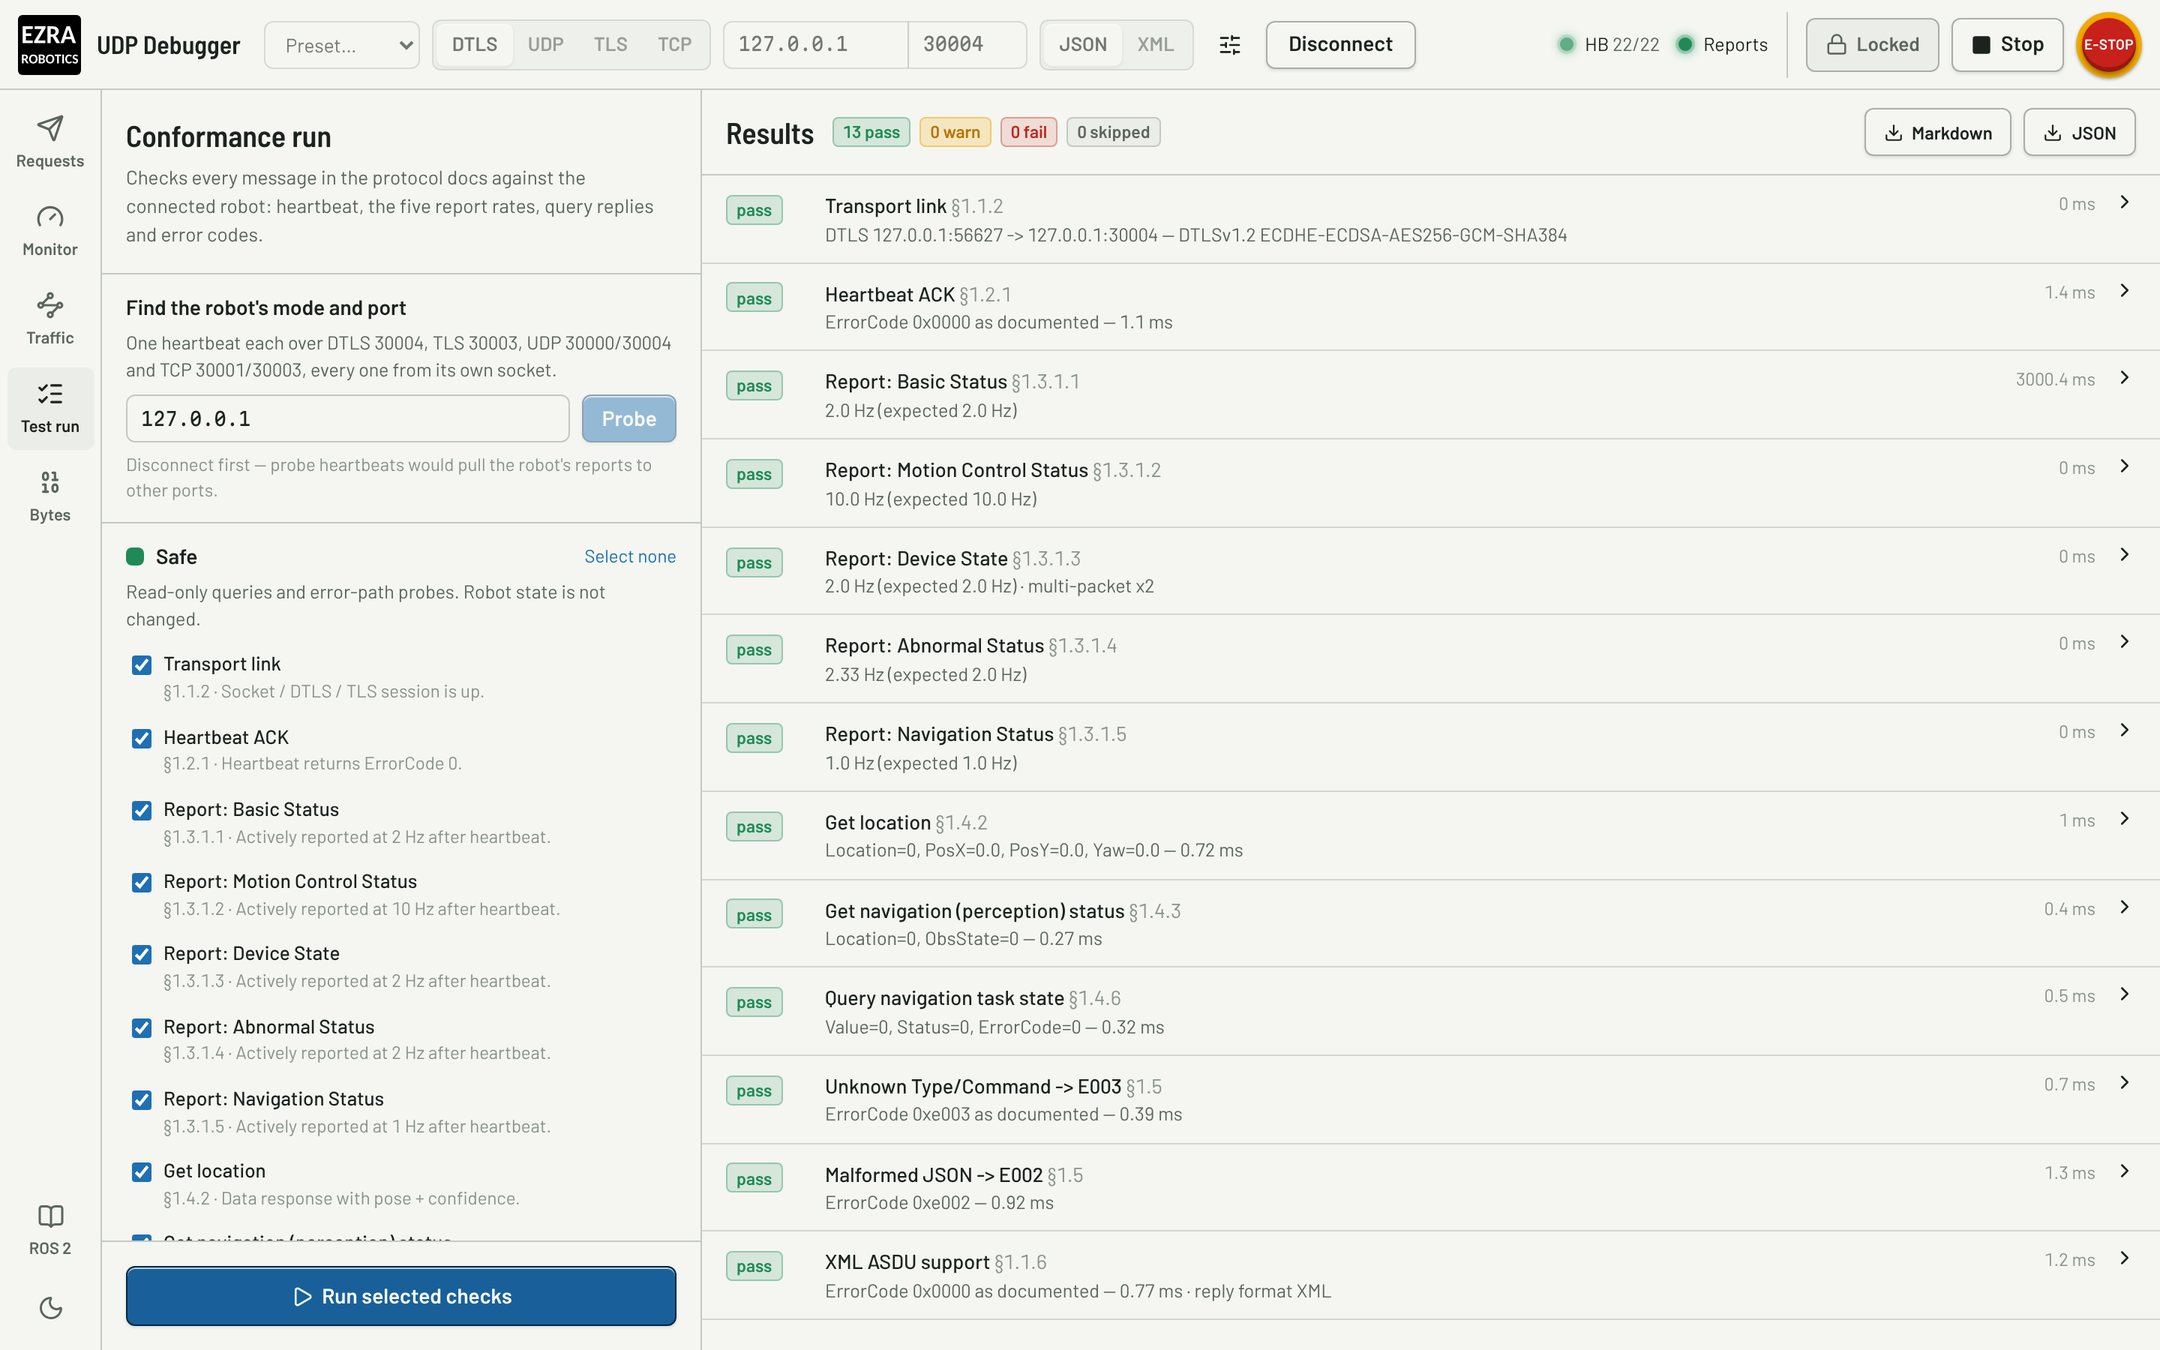
\includegraphics[width=\linewidth]{figures/gui-runner.jpg}
\caption{Conformance run: hasil per check, bisa diekspor ke Markdown/JSON.}
\end{figure}
Check dibagi tiga level. \textbf{Safe}: query dan uji error, robot tidak diubah. \textbf{Caution}: menerapkan
ulang mode/gait saat ini, mengembalikan lampu, membatalkan navigasi. \textbf{Motion}: berdiri, duduk, dan stream
axis --- butuh \ui{Armed}. Mencentang check \emph{caution} berarti kamu mengizinkannya.

\subsection{Bytes}
\begin{figure}[htbp]
\centering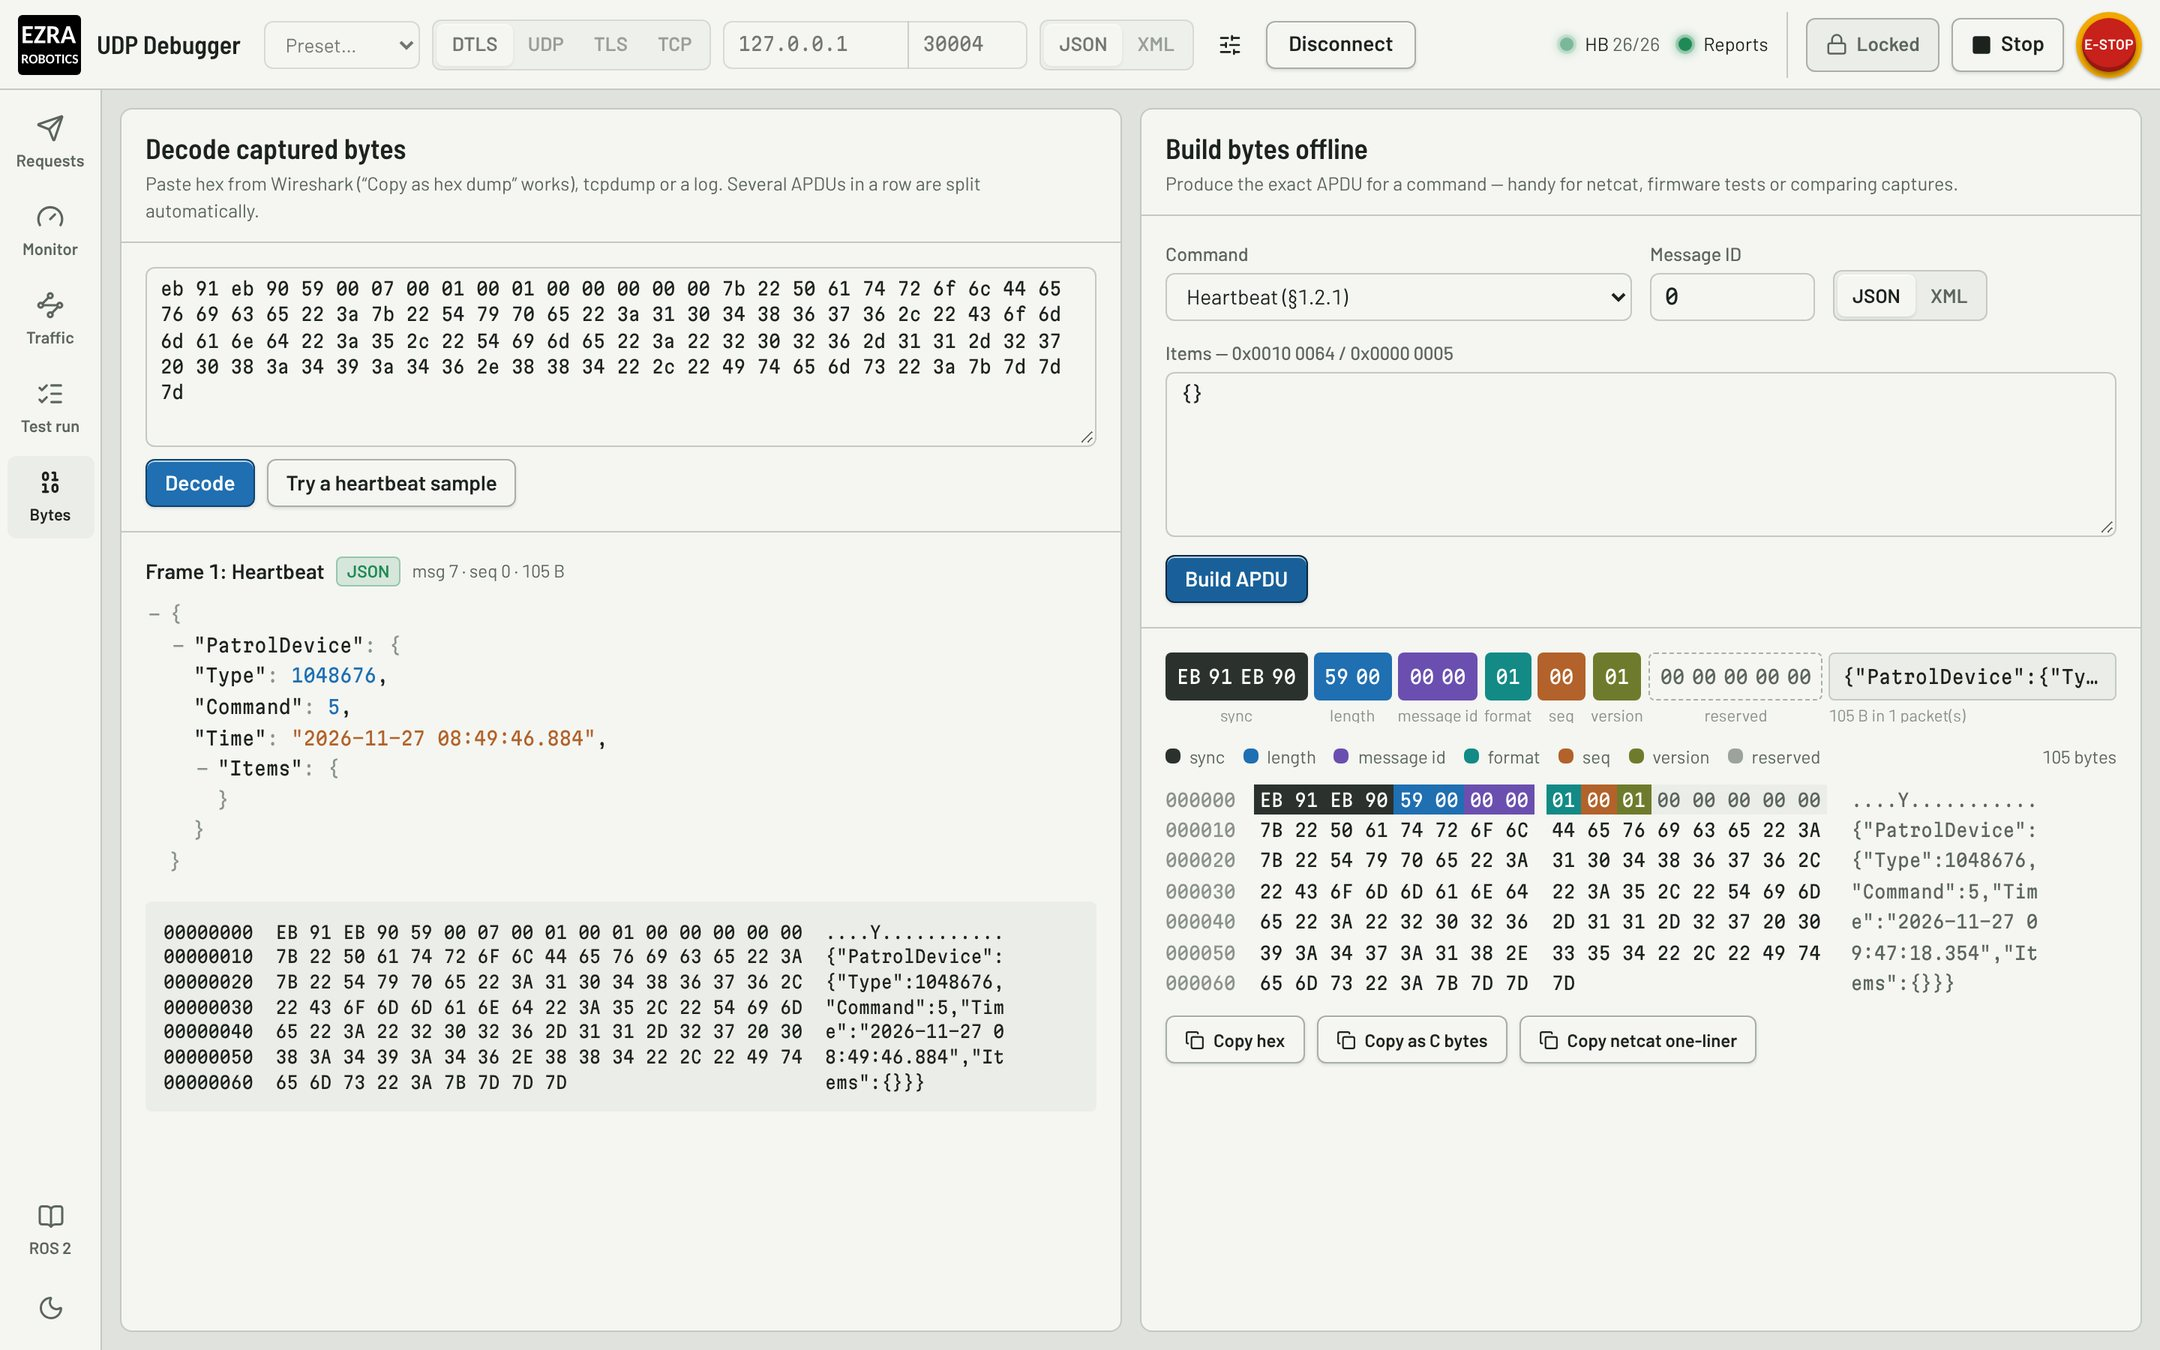
\includegraphics[width=\linewidth]{figures/gui-bytes.jpg}
\caption{Bytes: decode hex hasil capture dan membuat APDU secara offline.}
\end{figure}
Tempel hex dari Wireshark (\emph{Copy as Hex Dump} juga bisa) untuk di-decode --- beberapa APDU berurutan dipecah
otomatis. Encoder membuat APDU persis untuk command apa saja: \ui{Copy hex}, \ui{C bytes}, atau one-liner netcat.

% ======================================================================
\section{Panduan CLI}\label{sec:cli}
Semua perintah berbagi opsi koneksi: \code{-t dtls|udp|tls|tcp}, \code{-{}-host}, \code{-{}-port},
\code{-{}-xml}, \code{-{}-verify}, \code{-{}-ca}, \code{-{}-cert}, \code{-{}-key}, \code{-{}-compat}, \code{-{}-hb-hz},
\code{-{}-timeout}. Port default: DTLS 30004, TLS 30003, UDP 30000, TCP 30001.
\begin{xltabular}{\linewidth}{@{}L{60mm}Y@{}}
\toprule
\textbf{Perintah} & \textbf{Fungsi}\\\midrule
\endhead
\code{ezra-udp serve [-{}-mock] [-{}-open]} & API + GUI di :8765; \code{-{}-mock} = mock robot di proses yang sama\\
\code{ezra-udp mock [-{}-faults] [-{}-loss 0.05] [-{}-std]} & robot tiruan; fault setiap 15 detik, packet loss, versi STD\\
\code{ezra-udp probe -{}-host IP} & cari mode/port yang menjawab; exit 0 kalau ada yang \code{ok}\\
\code{ezra-udp list} & semua command + report beserta Type/Command\\
\code{ezra-udp send ID [-{}-items JSON]} & kirim satu command; yang menggerakkan robot butuh \code{-{}-yes}\\
\code{ezra-udp listen -s 10} & heartbeat + cetak report, lalu rate terukur\\
\code{ezra-udp suite [-{}-allow-caution] [-{}-allow-motion] [-{}-json out.json]} & conformance run; exit 1 kalau ada fail\\
\code{ezra-udp decode "eb 91 ..."} & decode hex (argumen atau stdin)\\
\bottomrule
\end{xltabular}
\begin{lstlisting}
ezra-udp probe --host 10.21.33.103
ezra-udp send location_get -t dtls
ezra-udp send gait --items '{"GaitParam": 4097}' -t tls
ezra-udp send motion_state --items '{"MotionParam": 1}' --yes      # robot berdiri
ezra-udp send nav_task --items '{"Item":[{"Value":1,"MapID":0,"PosX":0.5,"PosY":0,"PosZ":0,
  "AngleYaw":0,"PointInfo":1,"Gait":12290,"Speed":1,"Manner":0,"ObsMode":0,"NavMode":0}]}' \
  --yes --wait-deferred 120
ezra-udp suite -t dtls --allow-caution --json ~/Desktop/suite.json
\end{lstlisting}

% ======================================================================
\section{Prosedur pengecekan di pabrik}\label{sec:field}
Urutannya dari yang paling aman (jaringan, baca data) ke yang menggerakkan robot. Setiap tahap berisi
\emph{tujuan}, \emph{langkah}, \emph{lulus jika}, dan \emph{catat}. Isi checklist di Bab \ref{sec:checklist} sambil jalan.

\addcontentsline{toc}{subsection}{Tahap 0 --- Safety}
\begin{danger}[Tahap 0 --- Safety]
\begin{itemize}
\item Area kosong minimal 2 m di sekitar robot, lantai datar. Satu orang memegang remote + E-stop fisik.
\item GUI selalu \ui{Locked}, kecuali saat Tahap 9--10. Nilai kecepatan kecil: axis $\leq$ 0.2, velocity $\leq$ 0.2 m/s.
\item \ui{E-STOP} membuat robot lemas (damping) --- pastikan robot tidak di tangga atau tepi saat diuji.
\end{itemize}
\end{danger}

\tahap{Tahap 1 --- Jaringan}
\textbf{Tujuan:} Mac berada di subnet robot. \textbf{Langkah:}
\begin{enumerate}
\item Via kabel: \emph{System Settings \ra{} Network \ra{} (USB LAN) \ra{} Details \ra{} TCP/IP \ra{} Configure IPv4: Manually},
      IP \code{10.21.33.200}, subnet \code{255.255.255.0}, router \textbf{dikosongkan} (internet tetap lewat Wi-Fi).
      Via Wi-Fi robot: sambungkan ke SSID robot (DHCP).
\item Cek dari Terminal:
\begin{lstlisting}
ifconfig | grep "inet 10.21.33"           # IP Mac di subnet robot
ping -c 3 10.21.33.103
route -n get 10.21.33.103 | grep interface # harus interface ke robot, bukan Wi-Fi kantor
arp -a | grep 10.21.33                    # host lain di subnet (mis. host navigasi)
nc -vz 10.21.33.103 30003                 # port TLS terbuka?
\end{lstlisting}
\item Kalau macOS menampilkan pop-up firewall untuk Python, pilih \ui{Allow}.
\end{enumerate}
\textbf{Lulus jika:} ping dibalas dan rute lewat interface robot. \textbf{Catat:} IP Mac, interface, hasil \code{nc}.

\tahap{Tahap 2 --- Cari mode dan port}
\textbf{Langkah:} \code{make probe HOST=10.21.33.103} atau GUI \ui{Test run \ra{} Probe}. \textbf{Lulus jika:} minimal satu
baris \code{ok}. \textbf{Catat:} keenam baris (ambil screenshot), termasuk detail error baris yang gagal --- informasi ini
penting untuk Deep Robotics.

\tahap{Tahap 3 --- Connect, heartbeat, report}
\textbf{Langkah:} klik \ui{Use} di baris \code{ok} yang paling atas, lalu \ui{Connect}. \textbf{Lulus jika:} angka
\ui{HB} naik dan sama dengan jumlah terkirim; \ui{Reports} hijau dalam 2--3 detik. \textbf{Catat:} protokol/cipher
(\ui{Traffic \ra{} Engine log}), latensi heartbeat.

\tahap{Tahap 4 --- Identitas unit (Monitor)}
\textbf{Catat:} Model + Version (STD/PRO), baterai \% + voltase, suhu motor/driver tertinggi, utilisasi CPU kedua host,
status lidar/video, GPS fix, dan \textbf{rate kelima report} dibanding dokumen (2/10/2/2/1 Hz). Toleransi wajar
$\pm$40\%; di luar itu tetap dicatat.

\tahap{Tahap 5 --- Conformance run: safe}
\textbf{Langkah:} \ui{Test run}, centang semua \emph{safe}, \ui{Run selected checks}, lalu ekspor \ui{Markdown} + \ui{JSON}.
\textbf{Lulus jika:} semua \code{pass}. \code{warn} pada rate atau E00A (unit STD) dicatat, bukan dianggap gagal.

\tahap{Tahap 6 --- Conformance run: caution (robot diam)}
Centang check \emph{caution} lalu jalankan. Isinya: E004 (missing field), lampu kembali default, mode/gait saat ini
diterapkan ulang, dan pembatalan navigasi saat idle. \textbf{Catat} hasilnya.

\tahap{Tahap 7 --- Uji command satu per satu}
Kirim dari tab \ui{Requests}. Kolom ``cek'' menunjukkan apa yang harus berubah di \ui{Monitor}.
\begin{xltabular}{\linewidth}{@{}L{34mm}L{40mm}YL{9mm}@{}}
\toprule
\textbf{Command (\S)} & \textbf{Kirim} & \textbf{Harapan / cek} & \textbf{Lvl}\\\midrule
\endhead
Heartbeat 1.2.1 & otomatis & ErrorCode 0; HB acked = sent & safe\\
Usage mode 1.2.2 & Mode 0, 1, 2 & ErrorCode 0; Basic \code{ControlUsageMode} ikut; gait default mode ikut berubah & caut.\\
Motion state 1.2.3 & 1 Stand, 4 Sit, -2 damping & ErrorCode 0; \code{MotionState} berubah dalam beberapa detik & \textbf{gerak}\\
Gait 1.2.4 & 0x1001, 0x1003, 0x3002, 0x3003 & robot berdiri \& diam; \code{Gait} di Basic Status ikut berubah & caut.\\
Axis 1.2.5 & Hold to move X = 0.2 & mode Regular/Assist; robot jalan selama ditekan; \emph{tidak ada} balasan & \textbf{gerak}\\
Velocity 1.2.6 & Hold to move X = 0.1 & mode Navigation; \code{LinearX} $\approx$ 0.1; tidak ada balasan & \textbf{gerak}\\
Vel + position 1.2.7 & semua nol & hanya di gait six-axis; catat balasan (0 atau error) & \textbf{gerak}\\
Light effects 1.2.8 & CustomMode true, warna depan/belakang & lampu berubah; kembalikan dengan CustomMode false & safe\\
Charging 1.2.9 & Charge 1, lalu 0 & butuh docking station; \code{Charge}: goToPile \ra{} charging. Charge 2 hanya setelah fault & \textbf{gerak}\\
SDK mode 1.2.10 & SDKEnable, Frequency 100 & E007 kalau belum di-unlock --- itu sesuai dokumen & caut.\\
Sleep 1.2.11 & Sleep true lalu false & \code{Sleep}: 2 (entering) \ra{} 1 \ra{} 0 & caut.\\
Location init 1.4.1 & pose saat ini & \code{Relocation}: 0 running \ra{} 2 succeeded & caut.\\
Get location 1.4.2 & --- & data reply; cocok dengan Navigation Status & safe\\
Perception 1.4.3 & --- & Location + ObsState & safe\\
Nav task 1.4.4 & titik 0,5 m di depan & lihat Tahap 10 & \textbf{gerak}\\
Cancel nav 1.4.5 & saat idle / saat berjalan & 1 saat idle, 0 saat berjalan & caut.\\
Query nav 1.4.6 & --- & Value / Status / ErrorCode & safe\\
\bottomrule
\end{xltabular}

\tahap{Tahap 8 --- Uji error path}
Tujuannya memastikan robot menolak data salah dengan kode yang benar (\S1.5).
\begin{xltabular}{\linewidth}{@{}L{14mm}L{50mm}Y@{}}
\toprule
\textbf{Kode} & \textbf{Cara memicu} & \textbf{Catatan}\\\midrule
\endhead
E001 & Header \ra{} ASDU format byte = 2, atau body bukan JSON/XML & format tidak didukung\\
E002 & Body \ra{} raw mode \ra{} JSON terpotong (ada di conformance) & parse gagal\\
E003 & Custom message: Type 1048676, Command \code{0x00990099} & pesan tidak dikenal\\
E004 & Custom: Type 1048581, Command 2097154, Items \code{\{\}} & field hilang (lampu)\\
E005 & Motion state, raw body \code{"MotionParam": "x"} & tipe data salah --- \textbf{gerak} kalau robot menerimanya!\\
E006 & GUI dan CLI sama-sama mengirim axis dalam 2 detik & klien berbeda\\
E007 & SDK mode tanpa unlock & izin\\
E008 / E009 & Gait \code{1234} atau operasi yang tidak boleh di state saat ini & tergantung firmware\\
E00A & navigasi di unit STD & fitur tidak ada\\
header & version = 2, sync \code{EB 91 EB 91}, length salah & catat: dibalas E00x atau diabaikan\\
\bottomrule
\end{xltabular}

\addcontentsline{toc}{subsection}{Tahap 9 --- Uji gerak (Armed)}
\begin{warn}[Tahap 9 --- Uji gerak (Armed)]
\begin{enumerate}
\item Top bar \ui{Locked} \ra{} \ui{Armed}. Pastikan area aman.
\item Motion state \textbf{Stand}; tunggu sampai Monitor menunjukkan Stand.
\item Mode Regular: pilih Axis, \ui{Hold to move} dengan X = 0.2 selama $\pm$1 detik. Robot maju, lalu berhenti saat tombol dilepas.
\item Mode Navigation (Usage mode 1 atau gait 0x3002): Velocity X = 0.1 dengan hold to move. Cek \code{LinearX} di Monitor.
\item Gait switch saat robot diam; Sit; lalu uji \ui{Stop} (Esc) di tengah stream.
\item Uji \ui{E-STOP} sekali di posisi aman; catat waktu sampai \code{MotionState} = -2.
\item Kembali ke \ui{Locked}.
\end{enumerate}
\end{warn}

\tahap{Tahap 10 --- Navigasi (unit PRO, butuh peta)}
\begin{enumerate}
\item Get location: \code{Location} Normal (0) dan confidence $>$ 0.8. Kalau tidak, location init di pose yang diketahui.
\item Hitung titik 0,5 m di depan: $x' = x + 0{,}5\cos(\text{yaw})$, $y' = y + 0{,}5\sin(\text{yaw})$.
\item Usage mode Navigation, Stand, lalu Nav task: PosX $=x'$, PosY $=y'$, AngleYaw = yaw, PointInfo 1, Gait 12290,
      Speed 1 (low), NavMode 0 (straight), ObsMode 0.
\item Cek: balasan status langsung, Navigation Status 2 \ra{} 3 \ra{} 4, balasan hasil di \ui{Timeline}. Catat ErrorCode final.
\item Ulangi, lalu \ui{Cancel} saat Status = 3; cek ErrorCode 0 dan hasil ``cancelled''.
\end{enumerate}

\tahap{Tahap 11 --- ROS 2 topic (SSH)}
Ikuti Lampiran \ref{app:ros2}: source environment tanpa sudo, pastikan pesan \code{drdds} terbaca, jalankan script
health-check, lalu bandingkan \code{/MOTION\_INFO} dan \code{/fault\_aggregator} dengan report UDP di Monitor.

\tahap{Tahap 12 --- Rekam bukti}
\begin{lstlisting}
mkdir -p ~/Desktop/ezra-fieldtest && cd ~/Desktop/ezra-fieldtest
networksetup -listallhardwareports           # cari nama interface (mis. en7)
sudo tcpdump -i en7 -w robot-$(date +%H%M).pcap host 10.21.33.103   # Ctrl+C untuk stop
ezra-udp suite -t dtls --allow-caution --json suite.json
ezra-udp listen -s 30 -t dtls > listen.txt
\end{lstlisting}
Dari GUI: \ui{Traffic \ra{} Export} (JSON berisi data yang sudah didekripsi), \ui{Test run \ra{} Markdown/JSON}, dan
screenshot (\code{Cmd+Shift+4}). Capture DTLS/TLS terenkripsi --- isi paketnya ada di export Traffic.

\tahap{Tahap 13 --- Sebelum pulang}
Kembalikan robot ke kondisi awal (mode Regular, lampu default, sleep settings semula, Sit), lalu \ui{Disconnect}.
Lengkapi checklist dan tulis pertanyaan terbuka untuk Deep Robotics, misalnya port plain, sertifikat, perbedaan dengan
dokumen, atau kode error yang tidak terdokumentasi.

% ======================================================================
\section{Checklist lapangan}\label{sec:checklist}
Cetak bab ini. Isi \ok{} / \no{} dan catatan.

\subsection*{Unit \& koneksi}

\begin{tabularx}{\linewidth}{@{}l L{60mm}Y@{}}
\toprule
 & \textbf{Item} & \textbf{Hasil / catatan}\\\midrule
\cb & Model / versi (STD/PRO) / serial & \\
\cb & IP robot \& IP Mac / interface & \\
\cb & Ping + route OK & \\
\cb & Probe: mode/port yang \code{ok} & \\
\cb & Protokol/cipher (DTLS/TLS) & \\
\cb & Heartbeat ACK, latensi & \\
\bottomrule
\end{tabularx}

\subsection*{Report (rate terukur)}

\begin{tabularx}{\linewidth}{@{}l L{60mm}L{24mm}Y@{}}
\toprule
 & \textbf{Report} & \textbf{Spek} & \textbf{Terukur / catatan}\\\midrule
\cb & Basic Status & 2 Hz & \\
\cb & Motion Control Status & 10 Hz & \\
\cb & Device State (multi-packet?) & 2 Hz & \\
\cb & Abnormal Status & 2 Hz & \\
\cb & Navigation Status & 1 Hz & \\
\bottomrule
\end{tabularx}

\subsection*{Command}

\begin{tabularx}{\linewidth}{@{}l L{60mm}L{24mm}Y@{}}
\toprule
 & \textbf{Command} & \textbf{ErrorCode} & \textbf{Efek terlihat / catatan}\\\midrule
\cb & 1.2.1 Heartbeat & & \\
\cb & 1.2.2 Usage mode (0/1/2) & & \\
\cb & 1.2.3 Motion state (stand/sit/-2) & & \\
\cb & 1.2.4 Gait (4 nilai) & & \\
\cb & 1.2.5 Axis (no reply) & --- & \\
\cb & 1.2.6 Velocity (no reply) & --- & \\
\cb & 1.2.7 Velocity + position & & \\
\cb & 1.2.8 Light effects & & \\
\cb & 1.2.9 Autonomous charging & & \\
\cb & 1.2.10 Locomotion SDK & & \\
\cb & 1.2.11 Sleep settings & & \\
\cb & 1.4.1 Location init & & \\
\cb & 1.4.2 Get location & & \\
\cb & 1.4.3 Perception status & & \\
\cb & 1.4.4 Navigation task (final code) & & \\
\cb & 1.4.5 Cancel navigation & & \\
\cb & 1.4.6 Query navigation state & & \\
\bottomrule
\end{tabularx}

\subsection*{Error path \& format}

\begin{tabularx}{\linewidth}{@{}l L{60mm}Y@{}}
\toprule
 & \textbf{Uji} & \textbf{Kode yang diterima / catatan}\\\midrule
\cb & E001 format byte salah & \\
\cb & E002 JSON rusak & \\
\cb & E003 Type/Command tak dikenal & \\
\cb & E004 field hilang & \\
\cb & E005 tipe salah & \\
\cb & E006 dua klien & \\
\cb & E007 SDK tanpa unlock & \\
\cb & XML (format 0x00) & \\
\cb & Header: version/sync/length salah & \\
\bottomrule
\end{tabularx}

\subsection*{ROS 2 \& bukti}

\begin{tabularx}{\linewidth}{@{}l L{60mm}Y@{}}
\toprule
 & \textbf{Item} & \textbf{Hasil / catatan}\\\midrule
\cb & \code{/IMU} 200 Hz & \\
\cb & \code{/LIDAR/POINTS} 10 Hz (host robot) & \\
\cb & \code{/MOTION\_INFO} 20 Hz & \\
\cb & \code{/fault\_aggregator} $\approx$1 Hz & \\
\cb & \code{/CHARGE\_STATUS} & \\
\cb & Subscriber \code{/MOTION\_STATE}, \code{/GAIT}, \code{/NAV\_CMD} & \\
\cb & pcap, suite.json/md, traffic export, screenshot & \\
\bottomrule
\end{tabularx}

% ======================================================================
\section{Troubleshooting}\label{sec:trouble}
\begin{xltabular}{\linewidth}{@{}L{54mm}Y@{}}
\toprule
\textbf{Gejala} & \textbf{Penyebab \& solusi}\\\midrule
\endhead
\code{make setup}: ``Need Python $\geq$ 3.10'' & \code{brew install python@3.13}, lalu ulangi.\\
GUI: ``Backend is not running'' & Jalankan \code{make serve} / \code{make run}; halaman tersambung ulang sendiri.\\
``\emph{port 8765 is already in use}'' & EZRA sudah jalan di terminal lain: buka \code{http://127.0.0.1:8765}, atau hentikan yang lama (Ctrl+C).\\
``\emph{mock robot not started: \ldots{} already in use}'' & Mock lain masih jalan (\code{make demo} / \code{make mock}). Preset Mock tetap bisa dipakai dengan mock itu, atau hentikan dulu.\\
\code{ping} gagal & IP Mac bukan di \code{10.21.33.x}, kabel/adapter salah, atau Wi-Fi robot belum tersambung (Tahap 1).\\
Probe \code{unreachable} & Tidak ada rute: cek \code{route -n get 10.21.33.103}, kosongkan router di adapter LAN.\\
Semua \code{refused} & robotserver belum jalan, atau IP salah (mis. kamu ping host lain).\\
DTLS handshake timeout & Port salah atau enkripsi dimatikan --- jalankan probe; coba TLS 30003.\\
``\emph{probably a plain port}'' & Port menjawab tanpa enkripsi: pakai mode UDP/TCP plain di port itu.\\
``\emph{expects TLS}'' & Kamu mengirim TCP plain ke port TLS: pilih mode TLS.\\
``\emph{certificate problem}'' & Matikan verify, isi CA, atau minta sertifikat/kunci klien ke Deep Robotics.\\
``\emph{protocol/cipher mismatch}'' & Aktifkan \ui{Compat mode} (\code{-{}-compat}), coba lagi, lalu catat versi TLS robot.\\
HB acked 0, tapi terkoneksi (UDP) & Mode salah (UDP ke port DTLS), robot membalas dari port lain (matikan \emph{Connected UDP socket}), atau firewall Mac.\\
HB OK tapi \ui{No reports} & Report dikirim robot dari port lain: matikan \emph{Connected UDP socket}. Atau ada klien lain yang juga mengirim heartbeat (report pindah ke sana): hentikan klien lain.\\
\ui{Link lost} merah & Robot reboot, kabel/Wi-Fi putus, atau sesi DTLS direset --- \ui{Disconnect} lalu \ui{Connect}.\\
Rate report rendah & CPU robot sibuk (lihat Monitor), Wi-Fi lemah, atau paket hilang (UDP). Coba kabel.\\
\code{E006 Mismatched request client} & Klien lain mengirim axis dalam 2 detik terakhir; pakai satu klien saja.\\
\code{E00A Unsupported function} & Navigasi hanya ada di PRO.\\
\code{E007 No operation permission} & SDK mode belum di-unlock oleh after-sales.\\
Axis tidak menggerakkan robot & Robot belum Stand, mode bukan Regular/Assist, atau gait salah.\\
Velocity tidak berefek & Harus Navigation mode + Stand.\\
Nav task langsung gagal \code{0xA328} & Bukan Navigation mode. \code{0xA313}: lokalisasi bermasalah; \code{0xA341}: masih ada tugas berjalan.\\
Balasan ``matched by Type/Command only'' & Robot tidak mengembalikan message id yang sama; catat sebagai perbedaan dengan dokumen.\\
``incomplete multi-packet'' & Ada sub-paket yang hilang (UDP); kejadian sesekali wajar.\\
\bottomrule
\end{xltabular}

% ======================================================================
\section{Referensi}\label{sec:ref}

\subsection{Command}
\begin{xltabular}{\linewidth}{@{}L{12mm}YL{25mm}L{25mm}L{17mm}@{}}
\toprule
\textbf{\S} & \textbf{Command} & \textbf{Type} & \textbf{Command} & \textbf{Balasan}\\\midrule
\endhead
1.2.1 & Heartbeat & 0x0010 0064 & 0x0000 0005 & status\\
1.2.2 & Usage mode & 0x0010 0002 & 0x0050 0002 & status\\
1.2.3 & Motion state & 0x0010 0001 & 0x0020 0002 & status\\
1.2.4 & Gait & 0x0010 0001 & 0x0030 0002 & status\\
1.2.5 & Axis command & 0x0010 0001 & 0x0010 0002 & tidak ada\\
1.2.6 & Velocity command & 0x0010 0001 & 0x0011 0002 & tidak ada\\
1.2.7 & Velocity + position & 0x0010 0001 & 0x0012 0002 & status\\
1.2.8 & Light effects & 0x0010 0005 & 0x0020 0002 & status\\
1.2.9 & Autonomous charging & 0x0010 0004 & 0x0010 0002 & status\\
1.2.10 & Locomotion SDK & 0x0010 0005 & 0x0030 0002 & status\\
1.2.11 & Sleep settings & 0x0010 0002 & 0x0040 0002 & status\\
1.4.1 & Location init/reset & 0x0010 0003 & 0x0020 0002 & status\\
1.4.2 & Get location & 0x0010 0003 & 0x0020 0001 & data\\
1.4.3 & Perception status & 0x0010 0003 & 0x0011 0001 & data\\
1.4.4 & Navigation task & 0x0010 0003 & 0x0010 0002 & status + hasil\\
1.4.5 & Cancel navigation & 0x0010 0003 & 0x0010 0004 & data\\
1.4.6 & Query nav state & 0x0010 0003 & 0x0010 0001 & data\\
\bottomrule
\end{xltabular}

\subsection{Nilai enum penting}

\begin{tabularx}{\linewidth}{@{}L{34mm}Y@{}}
\toprule
\textbf{Field} & \textbf{Nilai}\\\midrule
Usage mode & 0 Regular, 1 Navigation, 2 Assist\\
Motion state & 1 Stand, 4 Sit, -2 soft emergency stop (damping)\\
Gait & 4097 (0x1001) Basic, 4099 (0x1003) Stair --- Regular; 12290 (0x3002) Flat, 12291 (0x3003) Stair --- Navigation\\
Light mode / color & 0 Solid, 1 Filling, 2 Moving, 3 Fading, 4 Breathing, 5 Flashing / 0 Black, 1 White, 2 Green, 3 Blue\\
Charge (request) & 0 stop, 1 start, 2 clear state (berisiko)\\
Nav status & 0 Idle, 1 exiting dock, 2 preprocessing, 3 navigating, 4 completed, 5 entering dock\\
Point info & 0 transition, 1 task, 2 stand, 3 charge, 4 stair\\
Speed / Manner / ObsMode / NavMode & 0 normal, 1 low, 2 high / 0 maju, 1 mundur / 0 aktif, 1 mati / 0 straight, 1 auto\\
Severity & 3 WARN, 4 ERROR, 5 FATAL\\
\bottomrule
\end{tabularx}

\subsection{Error umum (\S1.5)}

\begin{tabularx}{\linewidth}{@{}L{16mm}L{50mm}Y@{}}
\toprule
\textbf{Kode} & \textbf{Pesan} & \textbf{Keterangan}\\\midrule
0 & Success & \\
E001 & Unsupported data format & bukan XML/JSON\\
E002 & Data parsing failed & PatrolDevice/Items/Type/Command hilang atau rusak\\
E003 & Unsupported protocol type & Type/Command tidak dikenal\\
E004 & Missing necessary fields & field wajib hilang\\
E005 & Mismatched data type & tipe data salah\\
E006 & Mismatched request client & axis dalam 2 s dari klien lain\\
E007 & No operation permission & \\
E008 & Not allowed operation & \\
E009 & Operation failure & \\
E00A & Unsupported function & mis. navigasi di STD\\
E00B & Internal error & file internal gagal dibuka/diparse\\
\bottomrule
\end{tabularx}

\subsection{Error navigasi (Lampiran 1 dokumen)}
\begin{xltabular}{\linewidth}{@{}L{18mm}YL{18mm}Y@{}}
\toprule
\textbf{Kode} & \textbf{Arti} & \textbf{Kode} & \textbf{Arti}\\\midrule
\endhead
0x0000 & normal & 0xA34B & local nav: avoidance terus-menerus\\
0x2300 & selesai normal & 0xA34C & local planning gagal\\
0x2302 & dibatalkan user & 0xA34D & velocity navigasi tidak update\\
0x8605 & timeout menuju titik & 0xA34E & auto-charging berjalan, tugas ditolak\\
0xA301 & motion state abnormal & 0xA400 & gagal kirim titik ke local nav\\
0xA302 & baterai rendah & 0xA401 & gagal kirim titik ke global nav\\
0xA303 & motor abnormal & 0xA402 & gagal cancel local nav\\
0xA305 & LiDAR error & 0xA403 & gagal cancel global nav\\
0xA312 & planner tidak idle & 0xA404 & set parameter navigasi gagal\\
0xA313 & lokalisasi error & 0xA405 & local nav restart\\
0xA314 & terrain map error & 0xA406 & local nav: tidak ada obstacle map\\
0xA327 & gagal ganti gait & 0xA407 & local nav: tidak ada lokalisasi\\
0xA328 & bukan Navigation mode & 0xA408 & global nav restart\\
0xA341 & tugas masih berjalan & 0xA409 & global nav: tidak ada grid map\\
0xA343 & timeout keluar charging & 0xA40A & global nav: tidak ada lokalisasi\\
0xA344 & abnormal saat charging & 0xA40B & global planning gagal\\
0xA345 & auto-charging gagal & 0xA40C & titik target di obstacle\\
0xA349 & ganti peta gagal & 0xA40D--E & modul lokalisasi restart / sensor error\\
 & & 0xA40F & odometry publish time error\\
\bottomrule
\end{xltabular}

\subsection{Fault code (\S1.3.1.4 / \S2.5)}
\begin{xltabular}{\linewidth}{@{}L{18mm}YL{18mm}Y@{}}
\toprule
\textbf{Kode} & \textbf{Arti} & \textbf{Kode} & \textbf{Arti}\\\midrule
\endhead
0x8001 & motor overtemperature & 0x8109 & battery undertemperature\\
0x8002 & driver overtemperature & 0x810A & discharge overcurrent\\
0x8003 & driver overvoltage & 0x810D & charge overcurrent\\
0x8004 & driver undervoltage & 0x810E & output short circuit\\
0x8005 & driver overcurrent & 0x810F & IC error\\
0x8006 & driver communication & 0x8110 & MOSFET locked\\
0x8007 & driver status error & 0x8111 & data acquisition failure\\
0x8008 & driver operation anomaly & 0x8201 & IMU publish timeout\\
0x800A & joint high-speed terus-menerus & 0x8202 & IMU open failure\\
0x8012 & kabel sensor suhu putus & 0x8203 & IMU data timeout (joint)\\
0x8014 & batas posisi joint terlampaui & 0x8204 & IMU data invalid\\
0x8016 & data joint invalid & 0x8301 & CPU overtemperature\\
0x8017 & data joint tidak update & 0x8302 & CPU utilisasi tinggi\\
0x8101 & baterai rendah & 0x8303 & CPU frekuensi rendah\\
0x8102 & battery undervoltage & 0x8304 & memori tersisa sedikit\\
0x8104 & cell undervoltage & 0x8306 & file system hampir penuh\\
0x8105 & cell overvoltage & 0x8308 & inode hampir habis\\
0x8106 & pack overvoltage & 0x9401--03 & reflector positioning (dock)\\
0x8107 & pack undervoltage & 0x9406 & tidak ada arus dari dock\\
0x8108 & battery overtemperature & 0x9408--09 & obstacle saat undock / timeout ke dock\\
\bottomrule
\end{xltabular}

\subsection{Asumsi karena PDF terpotong}

\begin{tabularx}{\linewidth}{@{}L{48mm}Y@{}}
\toprule
\textbf{Hal} & \textbf{Yang dipakai tool}\\\midrule
Nilai format JSON & \code{0x01} (XML \code{0x00} terlihat)\\
Aturan multi-packet & gabung per (sumber, msg id, format) berurutan seq; sisa yang tidak lengkap dilaporkan setelah 1 s\\
Port plain & UDP 30000 / TCP 30001; probe juga mencoba 30004/30003\\
\code{BasicStatus.Charge} & 0--6 berurutan: idle, goToPile, charging, exitPile, error, onPiling, line\_charging\\
Nav status ``entering dock'' & 5\\
\code{ObsState} aktif & 1\\
Kode sukses navigasi & 0x0000 dan 0x2300 dianggap sukses\\
Balasan untuk query & data reply; tool juga menerima balasan status tambahan\\
\bottomrule
\end{tabularx}
Kalau perilaku robot berbeda dari tabel ini, catat di checklist --- itu temuan penting untuk Deep Robotics.

% ======================================================================
\appendix
\section{ROS 2 topic di robot}\label{app:ros2}
Topic (dokumen \S2, Lynx S10, ROS 2 Jazzy). Pesan \code{drdds/msg/*} adalah custom message Deep Robotics.

\begin{tabularx}{\linewidth}{@{}L{34mm}L{15mm}L{54mm}Y@{}}
\toprule
\textbf{Topic} & \textbf{Arah} & \textbf{Type} & \textbf{Rate / catatan}\\\midrule
\code{/IMU} & robot\ra & \code{sensor\_msgs/msg/Imu} & 200 Hz\\
\code{/LIDAR/POINTS} & robot\ra & \code{sensor\_msgs/msg/PointCloud2} & 10 Hz, hanya dari host robot\\
\code{/MOTION\_INFO} & robot\ra & \code{drdds/msg/MotionInfo} & 20 Hz\\
\code{/CHARGE\_STATUS} & robot\ra & \code{drdds/msg/StdStatus} & state + error\_code\\
\code{/fault\_aggregator} & robot\ra & \code{drdds/msg/FaultEventArray} & $\approx$1 Hz\\
\code{/NAV\_CMD} & dua arah & \code{drdds/msg/NavCmd} & 10 Hz; hanya Navigation mode\\
\code{/MOTION\_STATE} & \ra robot & \code{drdds/msg/MotionState} & butuh \code{motion\_master}\\
\code{/GAIT} & \ra robot & \code{drdds/msg/Gait} & 0x3002 / 0x3003\\
\bottomrule
\end{tabularx}

\subsection*{Langkah singkat}
\begin{lstlisting}
ssh <user>@10.21.33.103                 # tanpa sudo / su (dokumen: data tidak akan keluar)
source /opt/ros/jazzy/setup.bash
printenv | grep -E 'ROS_|RMW_|FASTRTPS|FASTDDS|CYCLONE'
ros2 interface list | grep drdds        # kosong? source workspace drdds:
find / -name 'MotionInfo.msg' -path '*drdds*' 2>/dev/null
ros2 daemon stop; ros2 daemon start
ros2 topic list -t
ros2 topic info -v /IMU                 # QoS publisher
ros2 topic hz /IMU
ros2 topic echo /MOTION_INFO
ros2 topic echo /LIDAR/POINTS --once --no-arr
ros2 topic echo /IMU --qos-reliability best_effort    # kalau echo diam
\end{lstlisting}

\subsection*{Script health-check (jalankan di robot)}
\begin{lstlisting}
cat > ~/ros2_topic_check.sh <<'EOF'
#!/usr/bin/env bash
set -u
DISTRO=${DISTRO:-jazzy}
source /opt/ros/$DISTRO/setup.bash
[ -n "${DRDDS_WS:-}" ] && source "$DRDDS_WS/install/setup.bash"
export PYTHONUNBUFFERED=1
ros2 daemon stop >/dev/null 2>&1; ros2 daemon start >/dev/null 2>&1
TOPICS=$(ros2 topic list 2>/dev/null)
rate() {
  local t=$1 exp=$2
  if ! grep -qx "$t" <<<"$TOPICS"; then printf "%-20s MISSING  expected %s Hz\n" "$t" "$exp"; return; fi
  local hz
  hz=$(timeout -s INT 6 ros2 topic hz "$t" 2>/dev/null | awk '/average rate/ {r=$3} END {print r}')
  if [ -z "$hz" ]; then printf "%-20s NO DATA  expected %s Hz\n" "$t" "$exp"
  else printf "%-20s OK %8.1f Hz (expected %s)\n" "$t" "$hz" "$exp"; fi
}
subs() {
  local n
  n=$(ros2 topic info "$1" 2>/dev/null | awk -F': ' '/Subscription count/ {print $2}')
  printf "%-20s subscribers=%s\n" "$1" "${n:-0}"
}
rate /IMU 200; rate /LIDAR/POINTS 10; rate /MOTION_INFO 20; rate /fault_aggregator 1
rate /CHARGE_STATUS "?"
subs /MOTION_STATE; subs /GAIT; subs /NAV_CMD
EOF
chmod +x ~/ros2_topic_check.sh && ~/ros2_topic_check.sh
\end{lstlisting}
Panduan lengkap (publish test, QoS, troubleshooting) ada di \code{docs/ROS2\_TOPIC\_DEBUG.md}.

\section{Struktur repo}\label{app:repo}
\begin{lstlisting}
backend/drds_udp/
  protocol/   header (APDU), asdu (JSON/XML), codes (tabel error/fault/nav), catalog (semua pesan)
  transport/  udp, dtls (pyOpenSSL memory BIO), stream (tcp/tls), tlsconf (compat, petunjuk error)
  engine/     session (msg id, heartbeat, link watchdog, stream, stop/E-STOP), reassembly, suite, probe
  server/     FastAPI REST + WebSocket, menyajikan web/out (+ mock robot opsional)
  mock/       robot tiruan (semua command, 5 report, device state multi-packet, nav task)
web/          GUI Next.js (static export)
scripts/      smoke.py: cek end-to-end untuk make smoke dan CI
docs/         ROS2_TOPIC_DEBUG.md, PROTOCOL_NOTES.md, manual/ (dokumen ini)
.github/      CI: test backend (Ubuntu + macOS), build GUI + smoke, build manual PDF
\end{lstlisting}
Setiap push dan PR menjalankan CI (\code{.github/workflows/ci.yml}): \code{pytest} di Ubuntu dan macOS dengan
Python 3.10 dan 3.13 (unit + end-to-end di keempat transport), CLI terhadap mock (\code{probe} + \code{suite} di
keempat transport), build + typecheck GUI, lalu \code{scripts/smoke.py -{}-gui}. Workflow \code{manual.yml}
membangun ulang PDF ini setiap kali \code{docs/manual/} berubah dan menyimpannya sebagai artifact.

\end{document}
